% !TEX root = perelman-geometry.tex
%!TEX TS-program = pdflatex
%!TEX encoding = UTF-8 Unicode


% epigraph for part 2

\cleardoublepage
\vspace*{\fill}
\begin{center}
\epigraph{\begin{minipage}{0.4\pagewidth} \textsf{The subject of mathematics is so serious that it is useful to seize the opportunity to make it a little entertaining.}\end{minipage}}{Blaise Pascal}
\end{center}
\vspace*{\fill}

\thispagestyle{empty}


\setchapterpreamble[o]{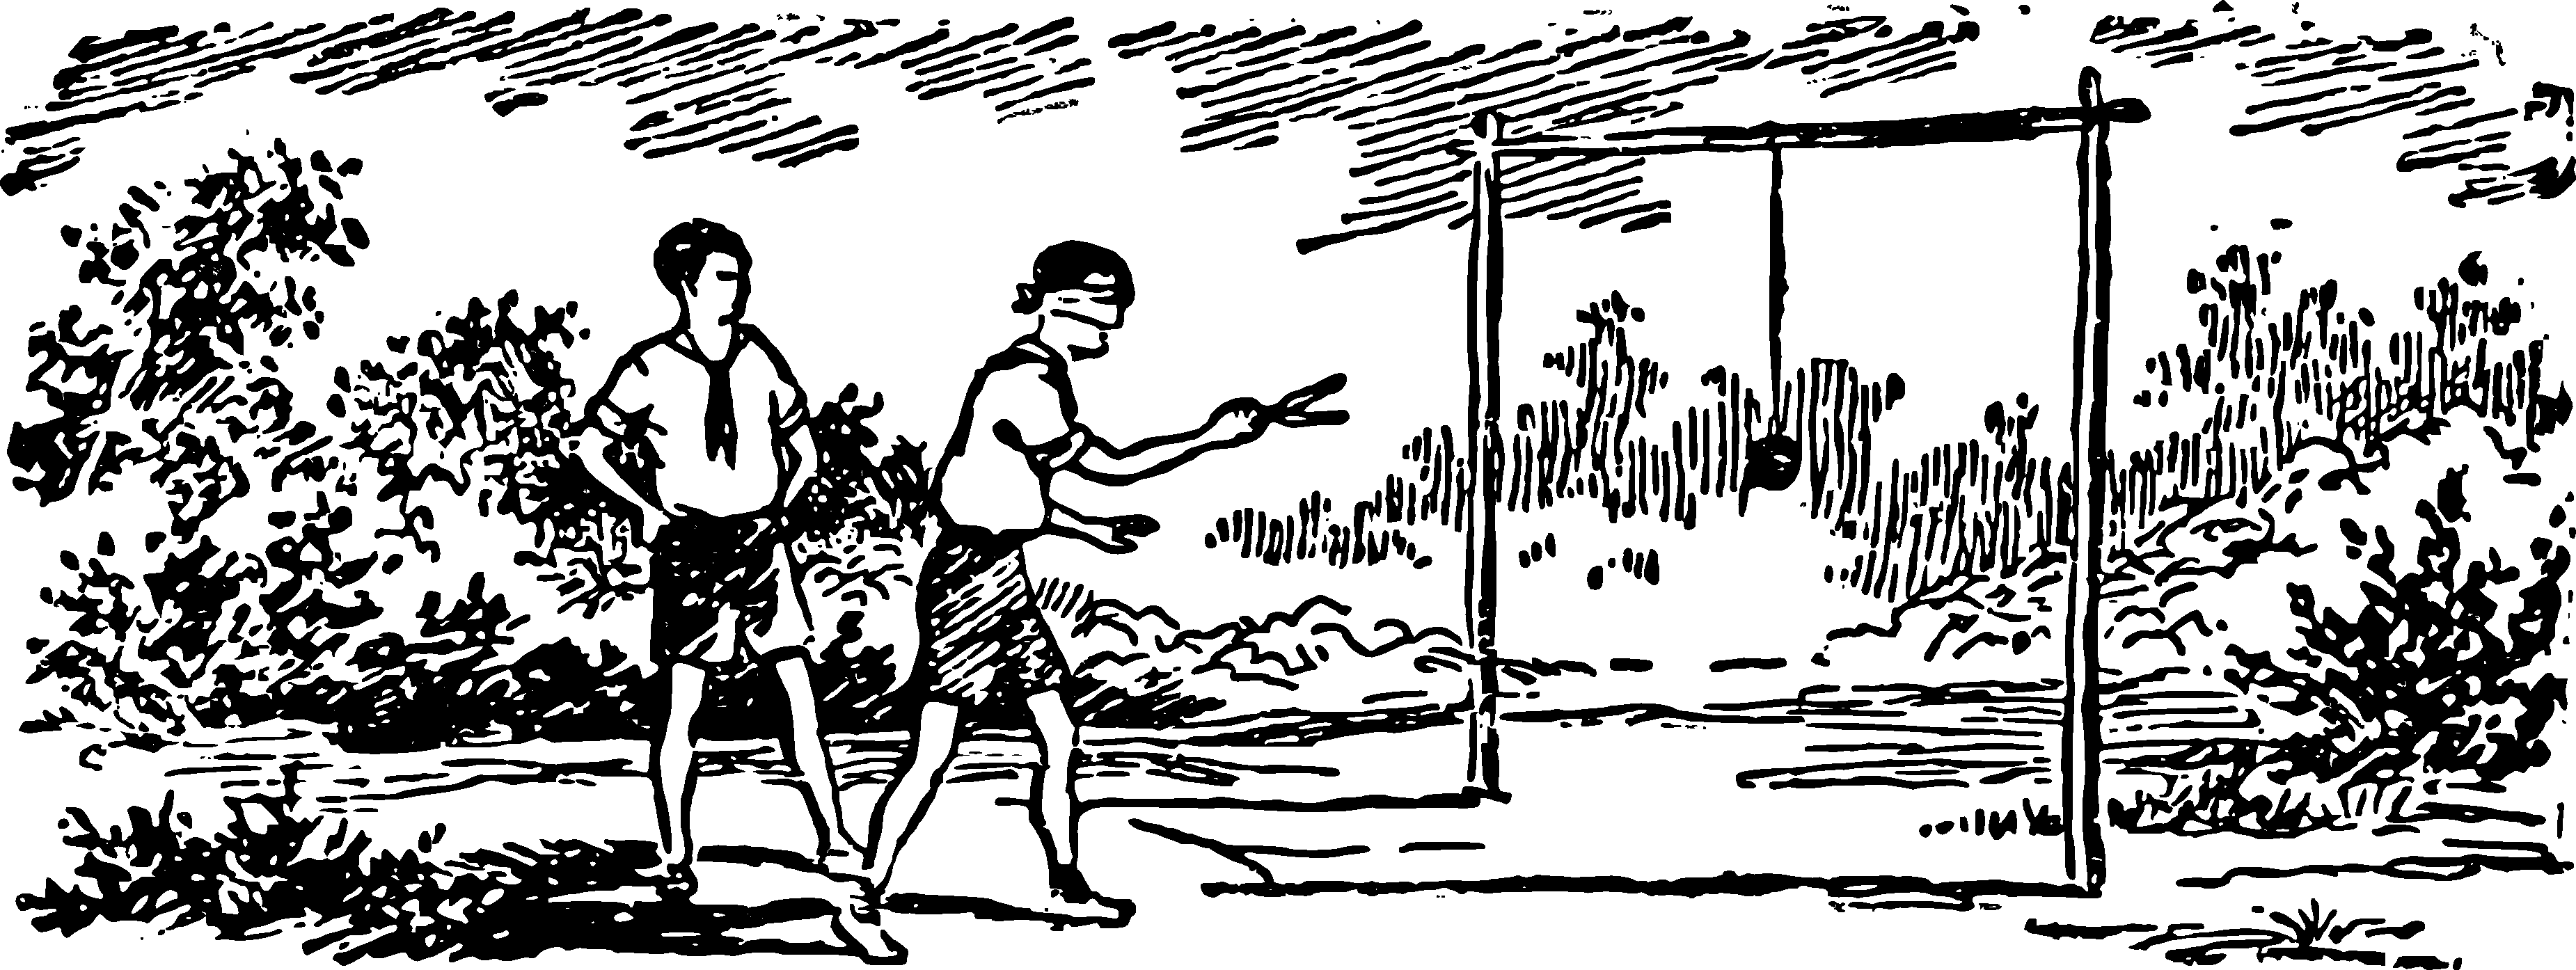
\includegraphics[width=1.2\textwidth]{figures/ch-08/fig-ch-08-head.pdf}\bigskip}

\chapter{Geometry In The Dark}
\label{ch-08}



\section{Into the Depths of the Hold}
\label{sec-8.1}

Let's transport ourselves from the open air of fields and sea to the cramped and dark hold of an old ship, where a young hero in one of Mayne Reid's novels successfully solved a geometric problem in an environment where, perhaps, none of our readers have ever had to do mathematics. In the novel \emph{The Boy Sailor} (or \emph{In the Depths of the Hold}), Mayne Reid tells the story of a young lover of sea adventures (Fig. 108), who, having no means to pay for his passage, sneaked into the hold of an unfamiliar ship and there unexpectedly found himself sealed in for the duration of the sea voyage. Rummaging through the luggage that filled his dungeon, he came across a crate of crackers and a barrel of water. The sensible boy understood that this limited supply of food and drink had to be used as sparingly as possible, and therefore decided to divide it into daily portions.

Counting the crackers was not difficult, but how to establish the portions of water without knowing its total supply? This was the problem facing Mayne Reid's young hero. Let's see how he coped with it.

\section{Measuring the Barrel}
\label{sec-8.2}

``I needed to establish a daily water ration for myself. To do this, I needed to find out how much water was in the barrel and then divide it into portions.''


``Fortunately, in the village school, the teacher taught us some basic information from geometry in arithmetic lessons: I had the concept of a cube, a pyramid, a cylinder, a sphere; I also knew that a barrel can be considered as two truncated cones stacked with their large bases.''

``To determine the capacity of my barrel, it was necessary to know its height (or, essentially, half of this height), then the circumference of one of the ends and the circumference of the midsection, i.e., the widest part of the barrel. Knowing these three quantities, I could accurately determine how many cubic units are contained in the barrel.''

\begin{figure}[h!]
\centering
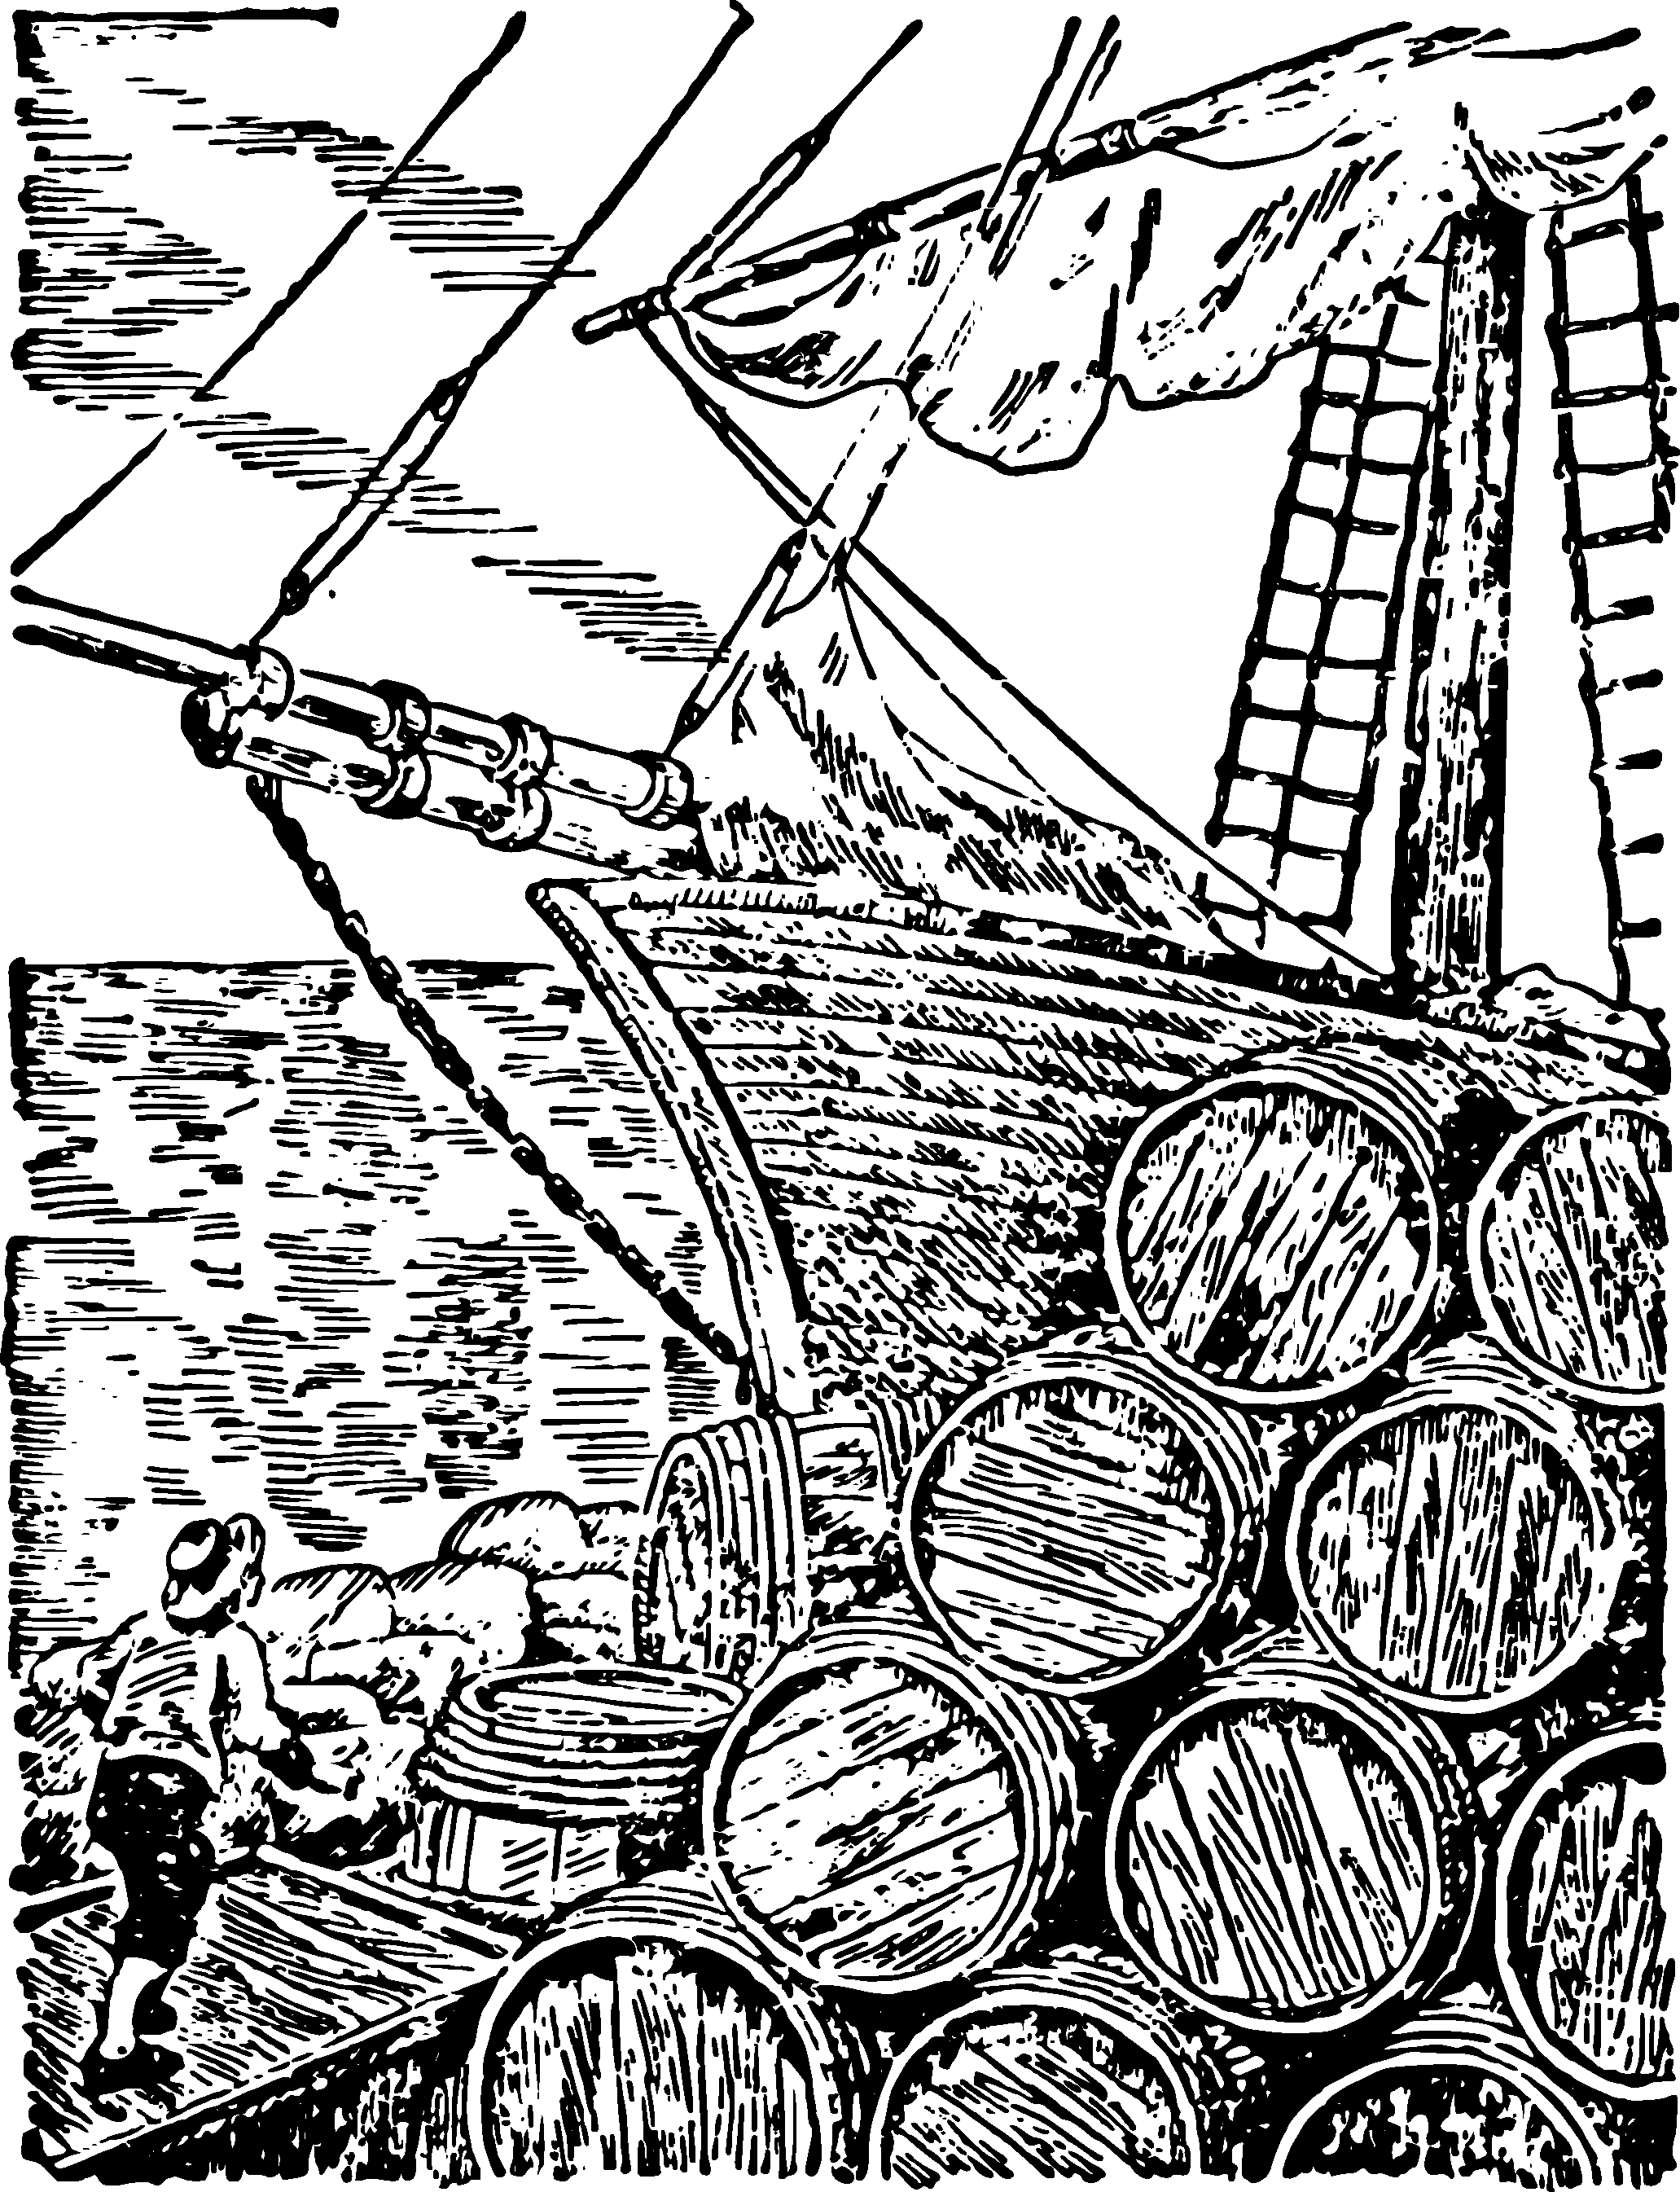
\includegraphics[width=0.7\textwidth]{figures/ch-08/fig-108.pdf}
\sidecaption[][-1cm]{The young adventurer from the novel by Mein-Reid.\label{fig-108}}
\end{figure}


``I needed to establish my daily water ration. To do this, I needed to find out how much water was in the barrel and then divide it into portions.''

``All I had to do was measure these quantities — but that's where all the difficulty lay.''

``How to perform these measurements?''

``Finding out the height of the barrel was not difficult: it was right in front of me; but as for the circumferences, I couldn't reach them. I was too short to reach the top; besides, there were boxes standing on the sides.''

``There was another difficulty: I had neither a scale nor a string that could be used for measurement; how could I determine the quantities if I had no measure? However, I decided not to give up my plan until I thought it through from all sides.''

\section{Measuring Ruler (The Mayne-Reid Problem)}
\label{sec-8.3}

``While contemplating the barrel, determined to measure it, I suddenly realised what I was lacking. A rod of sufficient length would assist me, one that could pass through the barrel at its widest point. If I inserted the rod into the barrel and pressed it against the opposite wall, I would know the diameter. Then, all I needed to do was triple the length of the rod to obtain the circumference. It's not perfectly precise, but it's sufficient for practical measurements. And since the hole I had previously made in the barrel was in its widest part, by inserting the rod into it, I would have the diameter I needed.''

``But where to find such a rod? It was not difficult. I decided to use a plank from a box of biscuits and immediately got to work. Indeed, the plank was only \SI{60}{\centi\meter} long, while the barrel was more than twice as wide. But this posed no problem; I just needed to prepare three sticks and tie them together to obtain a rod of sufficient length.''

``Cutting the plank along the grain, I prepared three well-rounded and smoothed sticks. How to bind them together? I used shoelaces from my shoes, each nearly a meter long. Tying the sticks together, I obtained a plank of sufficient length -- about one and a half meters.''

``I began to measure, but encountered a new obstacle. It was impossible to insert my rod into the 60-cm hole: the space was too tight. I couldn't bend the rod either -- it would likely break.''

``Soon I devised a way to insert my measuring rod into the barrel: I disassembled it into parts, inserted the first part, and then tied the second part to its protruding end; then, after pushing through the second part, I tied the third.''

``I positioned the rod so that it pressed against the opposite wall directly across from the hole and made a mark on it level with the surface of the barrel. Subtracting the thickness of the walls, I obtained the measurement necessary for my calculations.''

``I pulled out the rod in the same order as I inserted it, being careful to mark the places where the individual parts were tied together, so that later I could restore the rod to the same length it had in the barrel. A small error could result in a significant deviation in the final result.''

``So I had the diameter of the bottom base of the truncated cone. Now I needed to find the diameter of the barrel's top, which served as the upper base of the cone. I placed the rod on the barrel and pressed it against the opposite point of the edge, marking the diameter. It took no more than a minute.''

``All that remained was to measure the height of the barrel. You might say I could simply place a stick vertically next to the barrel and mark the height on it. But my space was quite dark, and when I placed the stick vertically, I couldn't see where the upper bottom of the barrel reached. I could only rely on touch. I would have to feel the barrel with my hands and the corresponding spot on the stick. Additionally, the stick, while rotating around the barrel, could tilt, giving me an incorrect measurement for the height.''


``After giving it some thought, I found a way to overcome this difficulty. I tied together only two planks, and I placed the third one on the top of the barrel so that it protruded beyond its edge by 30-40 cm; then I leaned a long rod against it to form a right angle with it and, consequently, be parallel to the height of the barrel. Making a mark at the point of the barrel that protruded the most, i.e., in the middle, and subtracting the thickness of the bottom, I thus obtained half of the barrel's height, or -- the same thing -- the height of one truncated cone.''

``Now I had all the necessary data to solve the problem.''

\section{What Needed to be Done}
\label{sec-8.4}

``Expressing the volume of the barrel in cubic units and then converting it into gallons\sidenote{A gallon is a measure of capacity. An English gallon contains 277 cubic inches (about 4.5 litres). There are 4 ``quarts'' in a gallon; 2 ``pints'' in a quart.} was a simple arithmetic calculation, which I could easily handle. True, I didn't have any writing materials for calculations, but they would have been useless anyway since I was in complete darkness. I often had to perform all four arithmetic operations mentally without pen and paper. Now I had to deal with not very large numbers, and the task didn't bother me at all.''

``But I encountered a new difficulty. I had three pieces of data: the height and both bases of the truncated cone; but what were the numerical values of these data? Before computing, I needed to express these values in numbers.''

``At first, this obstacle seemed insurmountable to me. Since I didn't have any feet, meters, or any measuring ruler, I thought I had to give up on solving the problem.''

``However, I remembered that in the port, I measured my height, which turned out to be four feet. How could this information be useful to me now? Quite simply: I could lay out four feet on my rod and use that as a basis for my calculations.''

``To mark my height, I stretched out on the floor, then placed the rod on myself so that one end touched my feet, and the other lay on my forehead. I held the rod with one hand and, with the other hand free, marked the spot on it opposite to where my temple was.''

``Further —— new difficulties. A rod equal to 4 feet is useless for measurement if it's not marked with small divisions -- inches. It's easy in theory to divide 4 feet into 48 parts (inches) and mark these divisions on the ruler. In practise, however, especially in the darkness I was in, it wasn't so easy and straightforward.''

``How to find the midpoint of these 4 feet on the rod? How to divide each half of the rod in half again, and then each of the feet into 12 inches, all precisely equal to each other?''

``I started by preparing a stick slightly longer than 2 feet. Comparing it with the rod, where 4 feet were marked, I found that the inch-length of the stick was slightly longer than 4 feet. Shortening the stick and repeating the operation several times, on the fifth attempt, I reached the point where the double length of the stick was exactly 4 feet.''

``This took a lot of time. But time was something I had plenty of: I was even glad to have something to fill it with.''

``However, I figured out how to streamline the process by replacing the stick with a string that could easily be folded in half. The shoelaces from my shoes came in handy for this. Tying them with a secure knot, I got to work — and soon I could cut a piece exactly 1 foot long. Folding it in half was easy. Folding it in thirds was harder. But I managed, and soon I had three pieces, each 4 inches long, in my hands. All that remained was to fold them in half again, and once more, to get a piece 1 inch long.''

``Now I had what I was earlier lacking to mark inch divisions on the rod; carefully aligning the pieces of my makeshift ruler, I made 48 notches representing inches. Then I had in my hands a ruler divided into inches, with which I could measure the lengths obtained. Only now could I complete the task.''

``I immediately set about this calculation. Measuring both diameters, I took the average of their lengths, then found the area corresponding to this average diameter. This gave me the size of the base of a cylinder equivalent to two cones of equal height. Multiplying these results by the height, I determined the cubic content of the sought-after volume.''

``Dividing the number of cubic inches obtained by 69 (the number of cubic inches in one quart)\sidenote{See the note on page~\pageref{sec-8.4}.}, I found out how many quarts were in my barrel.''

``It held over a hundred gallons -- 108, to be exact.''


\section{Verification of the Calculation}
\label{sec-8.5}


A reader knowledgeable in geometry will undoubtedly notice that the method used by the young hero Mayne-Reid to calculate the volume of two truncated cones is not entirely accurate. If (\figr{fig-109}) we denote the radius of the smaller bases as $r$, the radius of the larger base as $R$, and the height of the barrel, i.e., twice the height of each truncated cone, as $h$, then the volume obtained by the boy can be expressed by the formula:
\begin{figure}[h!]
\centering
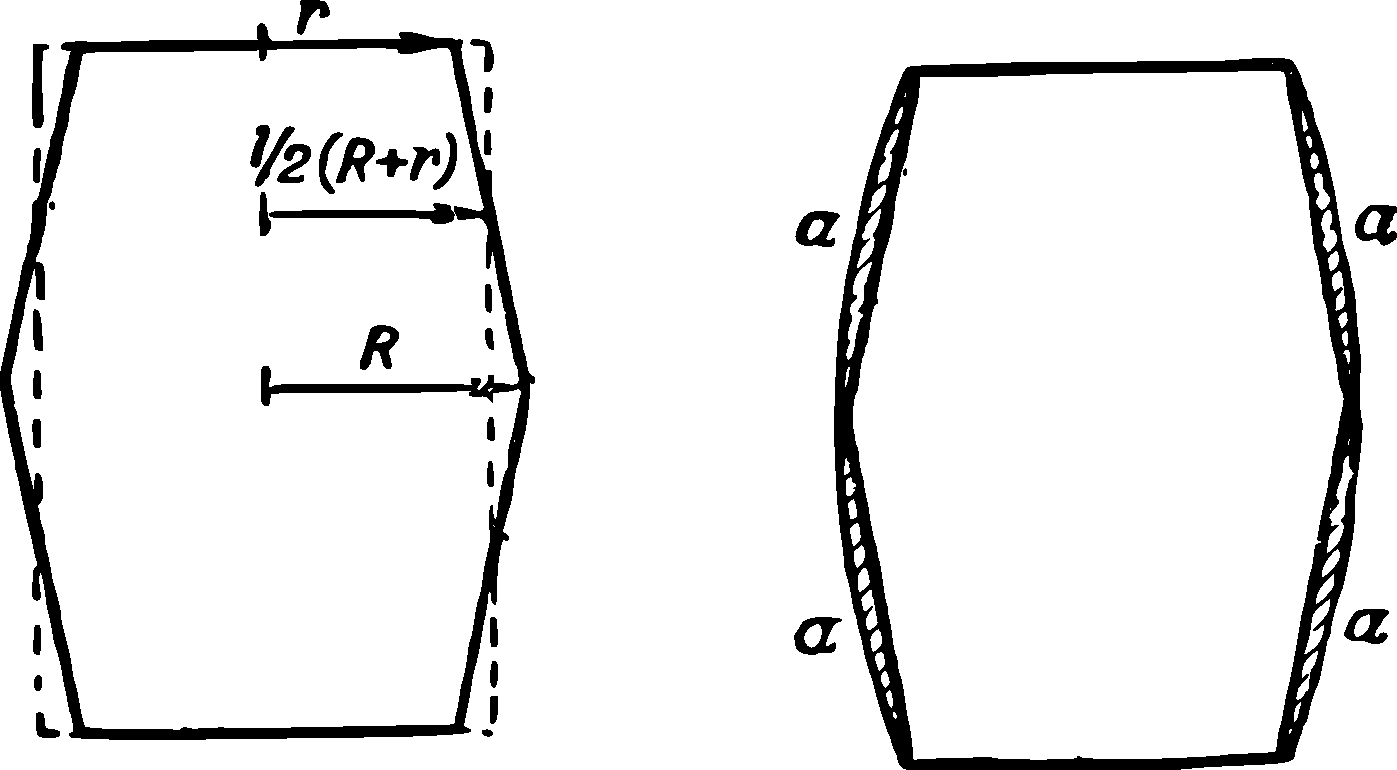
\includegraphics[width=0.8\textwidth]{figures/ch-08/fig-109.pdf}
\sidecaption{Checking the calculation of the young man.\label{fig-109}}
\end{figure}
\begin{equation*}%
\pi \left( \frac{R + r}{h} \right) h = \frac{\pi h}{4} (R^{2} + r^{2} + 2Rr).
\end{equation*}
However, following the rules of geometry, i.e., applying the formula for the volume of a truncated cone, we would obtain the expression for the sought-after volume:
\begin{equation*}%
\frac{\pi h}{3} (R^{2} + r^{2} + Rr).
\end{equation*}
Both expressions are not identical, and it is easy to see that the second one is greater than the first by:
\begin{equation*}%
\frac{\pi h}{12} (R - r)^{2}.
\end{equation*}
Those familiar with algebra will understand that the difference  $(πh/12) \, (R - r)^{2}$ is a positive quantity. That is, the method used by the Mayne-Reid boy resulted in an underestimated result.

It is interesting to determine approximately how much this underestimation is. Barrels are usually designed in such a way that their maximum width exceeds the diameter of the base by \nicefrac{1}{5}, i.e., $R - r = R/5$.

Assuming that the barrel in the Mayne-Reid novel was of this shape, we can find the difference between the obtained and the true volume of the truncated cones:
\begin{equation*}%
\frac{\pi h}{12} (R - r)^{2} = \frac{\pi h}{12} \left(\frac{R}{5}\right)^{2} = \frac{\pi hR^{2}}{300}.
\end{equation*}
That is, approximately $hR^{2}/300$ (if we consider $\pi \approx 3 $). The error is equal to, as we see, the volume of the cylinder whose base radius is the radius of the largest section of the barrel, and its height is one three-hundredth of its height.

However, this does not reflect the true result, as the volume of the barrel is inherently greater than the volume of the two truncated cones inscribed within it. This is evident from \figr{fig-109} (right), where it can be seen that with the specified method of measuring the barrel, a part of its volume, denoted by the letters $a$, $a$, $a$, $a$, is disregarded.


The young mathematician Mayne-Reid did not invent this formula for calculating the volume of a barrel; it is presented in some elementary geometry manuals as a convenient method for approximate determination of barrel contents. It's worth noting that measuring the volume of a barrel with absolute precision is a very difficult task. This was contemplated by the great Kepler himself, who left in his mathematical works a special study on the art of measuring barrels. A simple and precise geometric solution to this problem has not been found to this day: there are only established practical methods that provide results with greater or lesser approximation. For instance, in southern France, a simple formula, well justified by experience, is used:
\begin{equation*}%
\text{Volume of barrel} = 3.2\, hRr, 
\end{equation*}
where: $h$ is the height of the barrel, $R$ is the radius of the larger base, $r$ is the radius of the smaller base.

It is also interesting to consider the question: why, in fact, barrels are given such an inconvenient shape for measuring -- a cylinder. with bulging sides? Wouldn't it be easier to make strictly cylindrical barrels? Such cylindrical barrels, however, are made, but not wooden, but metal (for kerosene, for example). So, in front of us:

\ques Why are wooden barrels made with convex sides? What is the advantage of this shape?

\ans The benefit lies in the fact that by fitting hoops onto the barrels, they can be tightened tightly and securely by a very simple method: by pushing them closer to the wider part. Then the hoop can be easily tightened around the staves, providing the barrel with the necessary strength.

For the same reason, wooden buckets, tubs, vats, etc., are usually given a shape not of a cylinder, but of a truncated cone: here too, tight fitting of hoops around the product is achieved simply by pushing them onto the wider part (\figr{fig-110}).

\begin{figure}[h!]
\centering
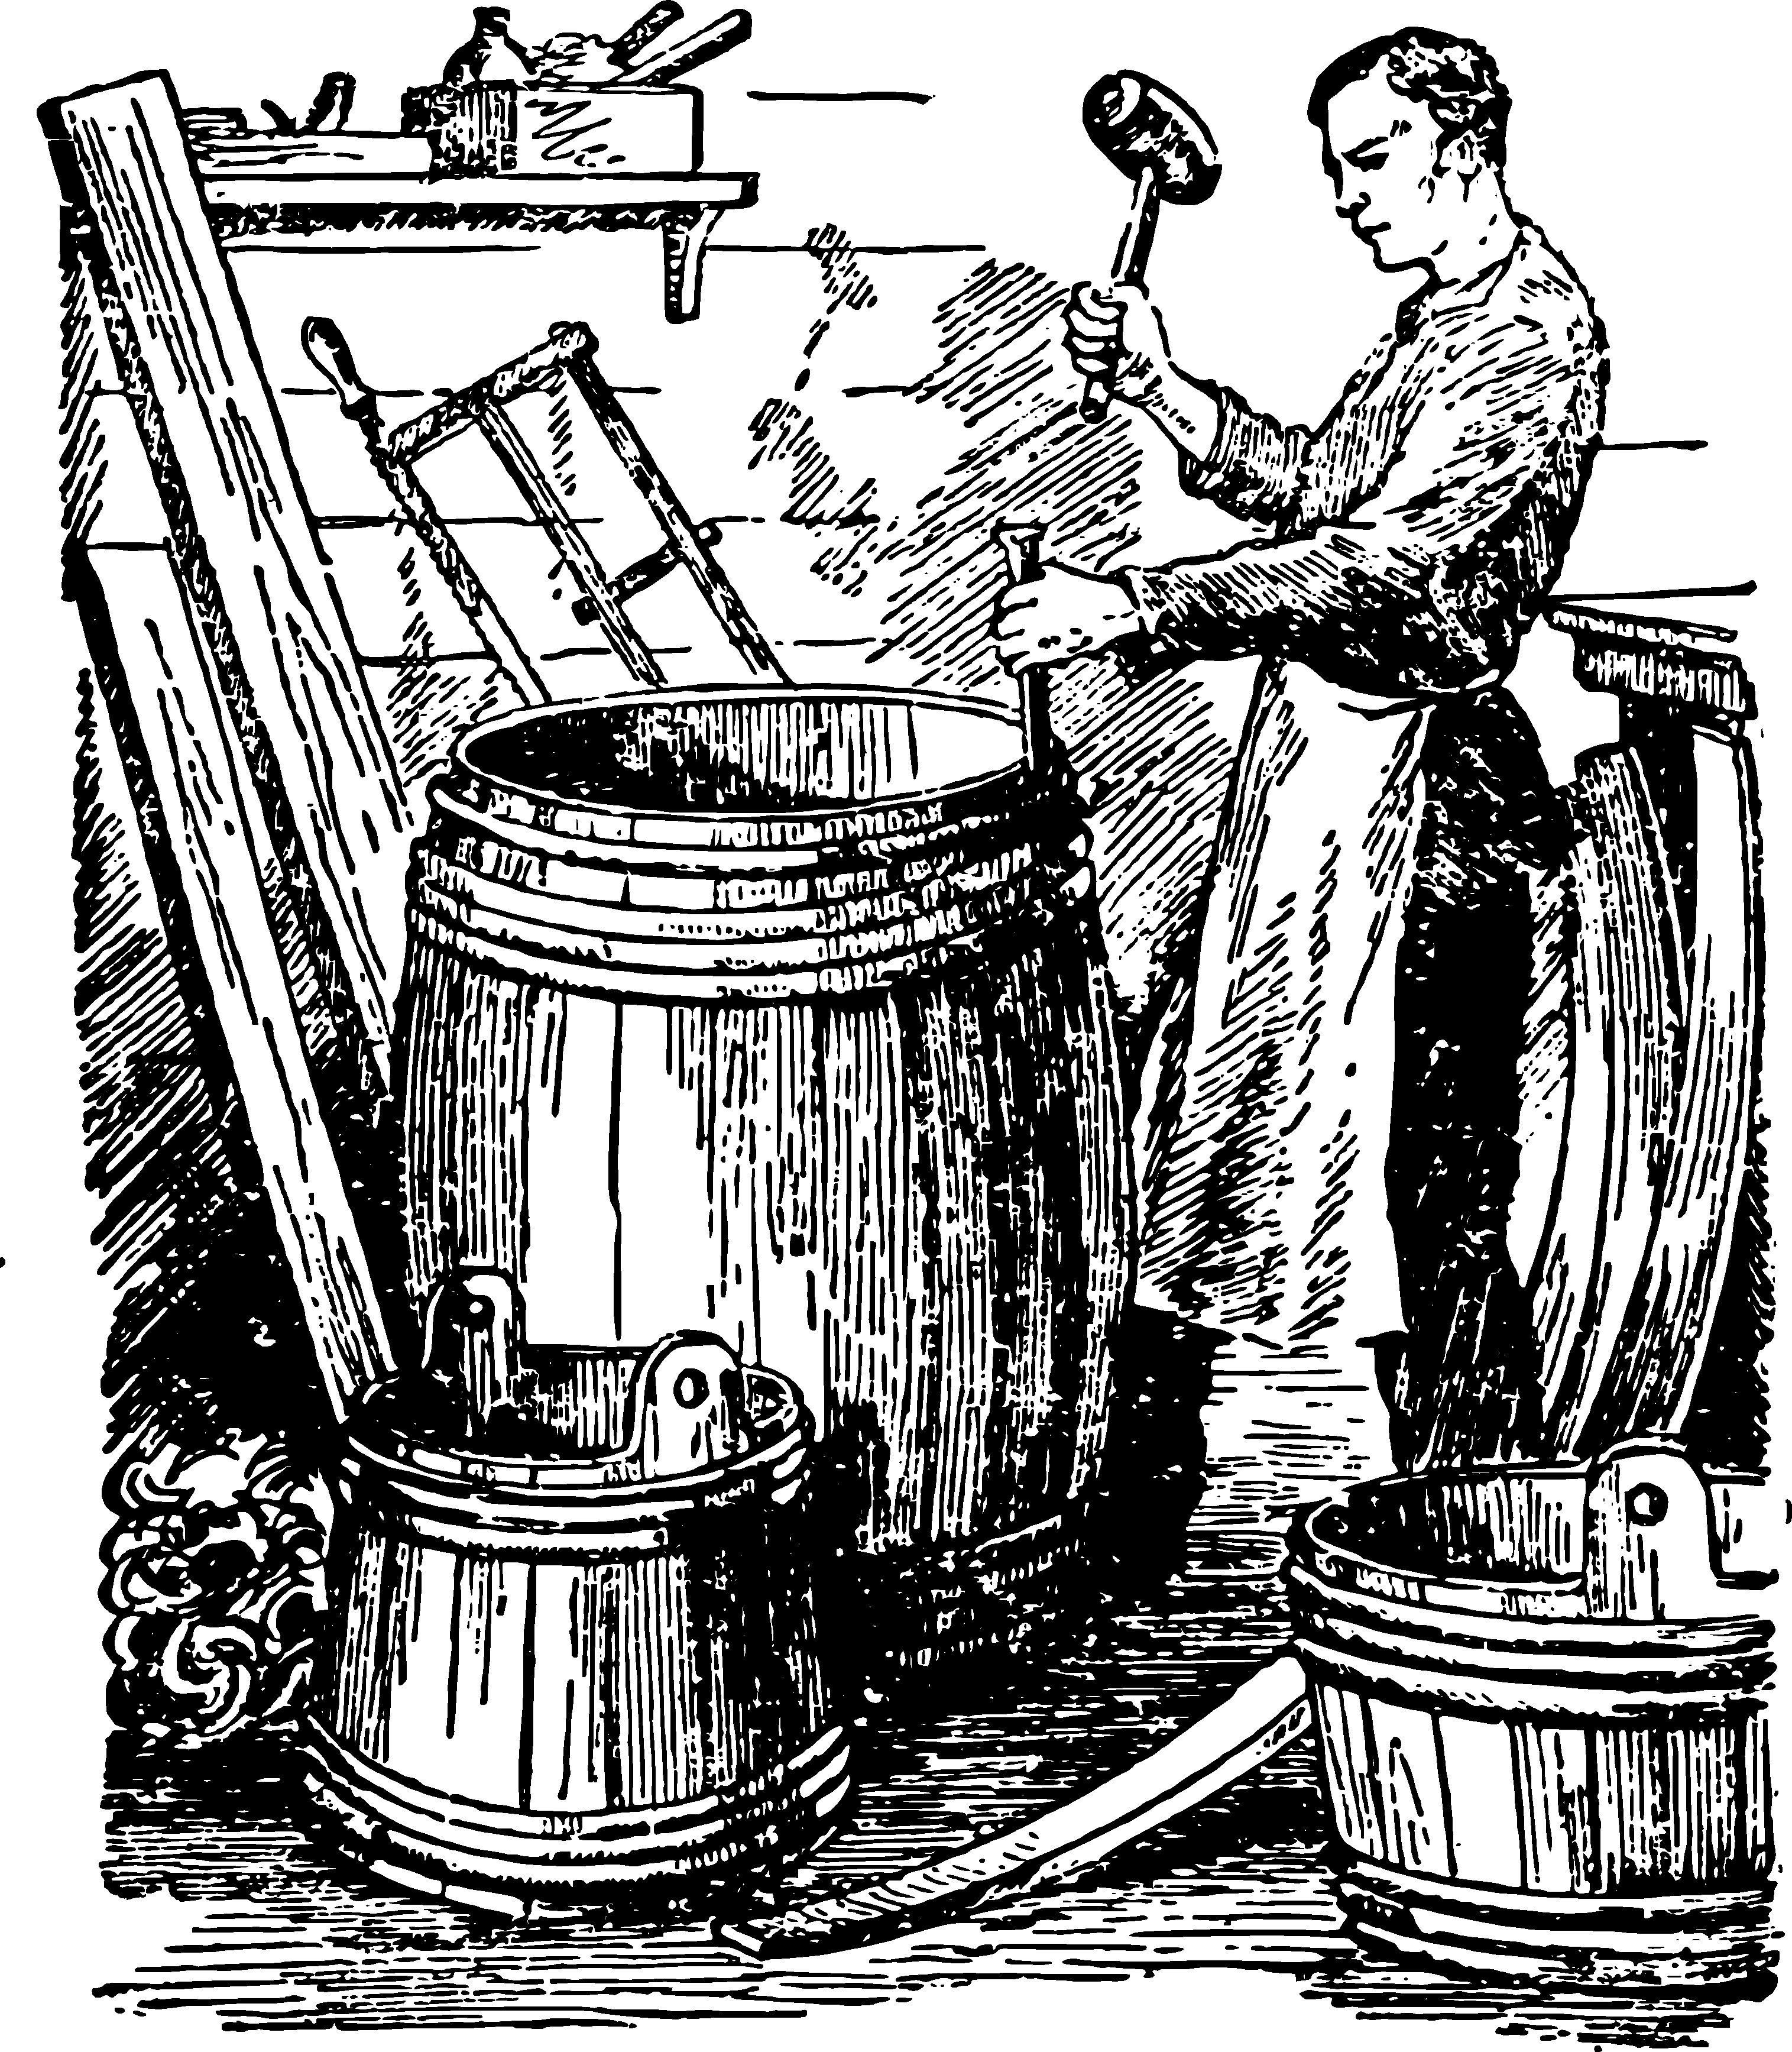
\includegraphics[width=0.7\textwidth]{figures/ch-08/fig-110.pdf}
\sidecaption[][-2cm]{Tight wrapping of the barrel with hoops is achieved by pushing them over a wide part.\label{fig-110}}
\end{figure}

Here it would be appropriate to acquaint the reader with the opinions on this subject expressed by Johannes Kepler. In the period between the discovery of the 2nd and 3rd laws of planetary motion, the great mathematician devoted attention to the question of the shape of barrels and even compiled a whole mathematical treatise on this topic. Here is how this is called: \emph{Stereometry of Barrels}: 

\begin{quote}
Wine barrels have been assigned a round shape according to the requirements of the material, construction, and use. The liquid, when kept in metal vessels for a long time, spoils due to rust; glass and clay are inadequate in size and unreliable; stone vessels are unsuitable for use due to their weight—thus, wines remain to be poured and stored in wooden barrels. From a single whole log, it is also not easy to prepare vessels large enough and in sufficient quantities, and even if it is possible, they crack. Therefore, barrels should be constructed from many pieces of wood connected to each other, and it is impossible to prevent the leakage of liquid through the gaps between individual pieces neither by using any material nor by any other method except compressing them with bindings\dots{}

If it were possible to construct vessels resembling spheres from wooden planks, then spherical vessels would be the most desirable. But since it is impossible to compress the planks into a sphere with bindings, a cylinder takes its place. But this cylinder cannot be perfectly smooth because weakened bindings would immediately become useless and could not be tightened any stronger, if the barrel did not have a conical shape, tapering on both sides from its belly. This shape is convenient for rolling and transportation in carts and, consisting of two similar halves on a common base, it is the most advantageous for rocking and aesthetically pleasing.\sidenote{It should not be assumed that Kepler's treatise on measuring barrels is a mathematical triviality, a pastime of genius during leisure hours. No, it is a serious work in which infinitesimal quantities and the principles of integral calculus are introduced into geometry for the first time. The wine barrel and the practical problem of measuring its capacity served as an occasion for him to engage in deep and fruitful mathematical reflections. The translation of \emph{Stereometry of Wine Barrels} was published in 1935.}
\end{quote}

\section{The Night Journey of Mark Twain}
\label{sec-8.6}

The resourcefulness shown by the boy from the Mayne Reid story in his dire situation is truly remarkable. In the pitch darkness he found himself in, most people wouldn't even be able to orient themselves properly, let alone perform any measurements or calculations. It is instructive to compare Reid's story with a humorous tale of aimless wandering in a dark hotel room, an adventure seemingly experienced by the famous compatriot of Mayne Reid, the humorist Mark Twain. This story effectively highlights how difficult it is to form a correct understanding of the layout of objects in the dark, even in an ordinary room, if the environment is unfamiliar. Below is a condensed rendition of this amusing episode from \emph{The Innocents Abroad} by Mark Twain.

\begin{quote}
I woke up and felt thirsty. A wonderful idea occurred to me -- to get dressed, go out to the garden, and refresh myself by washing up at the fountain.

I got up slowly and started searching for my things. Found one sock. Where the other one was, I couldn't imagine. Carefully lowering myself to the floor, I began to feel around, but to no avail. I searched further, groping and scooping. I moved further and further, but couldn't find the sock and only bumped into furniture. When I went to bed, there was much less furniture around; now the room was full of it, especially chairs, which seemed to be everywhere. Had two more families moved in during this time? I hadn't seen any of these chairs in the darkness, but kept bumping my head into them.

Finally, I decided I could live without one sock. Standing up, I headed towards the door, or so I thought -- but unexpectedly saw my dim reflection in the mirror.

It was clear that I was lost and had no idea where I was. If there had been just one mirror in the room, it would have helped me orient myself, but there were two, and that was just as bad as a thousand.

I wanted to make my way to the door along the wall. I began my attempts again -- and knocked over the picture. The noise was not great, but it sounded as loud as a whole panorama. Harris (my roommate, sleeping in the other bed) didn't move, but I felt that if I continued in the same manner, I would definitely wake him up. I'll try another way. I'll find the round table again -- I had been near it several times -- and from there, I'll try to make my way to my bed; if I find the bed, I'll find the pitcher of water, and then, at least, I'll quench my unbearable thirst. It's best to crawl on hands and knees; I had already tried this method and trusted it more.

Finally, I managed to stumble upon the table -- felt it with my head -- with a relatively small noise. Then I stood up again and walked, balancing with my arms outstretched and fingers spread. Found a chair. Then a lamp. Another chair. Then a sofa. My stick. Another sofa. This surprised me; I knew perfectly well that there was only one sofa in the room. Stumbled upon the table again and received a new blow. Then bumped into a new row of chairs.

It was only then that it occurred to me, as it should have long ago: the table was round and therefore could not serve as a starting point for my wanderings. By chance, I went into the space between the chairs and the sofa -- but found myself in an entirely unfamiliar area, dropping the candlestick by the fireplace along the way. After the candlestick, I dropped the lamp, and after the lamp, the decanter crashed to the floor with a clang.

``Ah,'' I thought, ``finally found you, my dear!''

``Thieves! Robbers!'' yelled Harris.

The noise and cries woke up the entire house. The owner, guests, and servants appeared with candles and lanterns.

I looked around. It turned out I was standing next to Harris's bed. Only one sofa was against the wall; only one chair was positioned to bump into -- I circled around it like a planet, colliding with it like a comet for a whole half of the night.

After checking my pedometer, I confirmed that I had covered 47 miles during the night.
\end{quote}

The last statement is exaggerated beyond measure: it is impossible to walk 47 miles on foot in just a few hours. However, the other details of the story are quite plausible and accurately depict the comedic difficulties one typically encounters when wandering aimlessly and haphazardly in the darkness of an unfamiliar room. Moreover, we should especially appreciate the remarkable methodical approach and the spirit of the young hero, Mayne-Reid, who not only managed to orient himself in complete darkness but also solved a challenging mathematical problem under such conditions.


\section{Mysterious Circumnavigation}
\label{sec-8.7}


Regarding Twain's circling in the dark room, it's interesting to note a mysterious phenomenon observed in people wandering with their eyes closed: they cannot walk in a straight line but invariably veer off to the side, describing an arc, while imagining that they are moving straight ahead (see \figr{fig-111}).


\begin{figure}[h!]
\centering
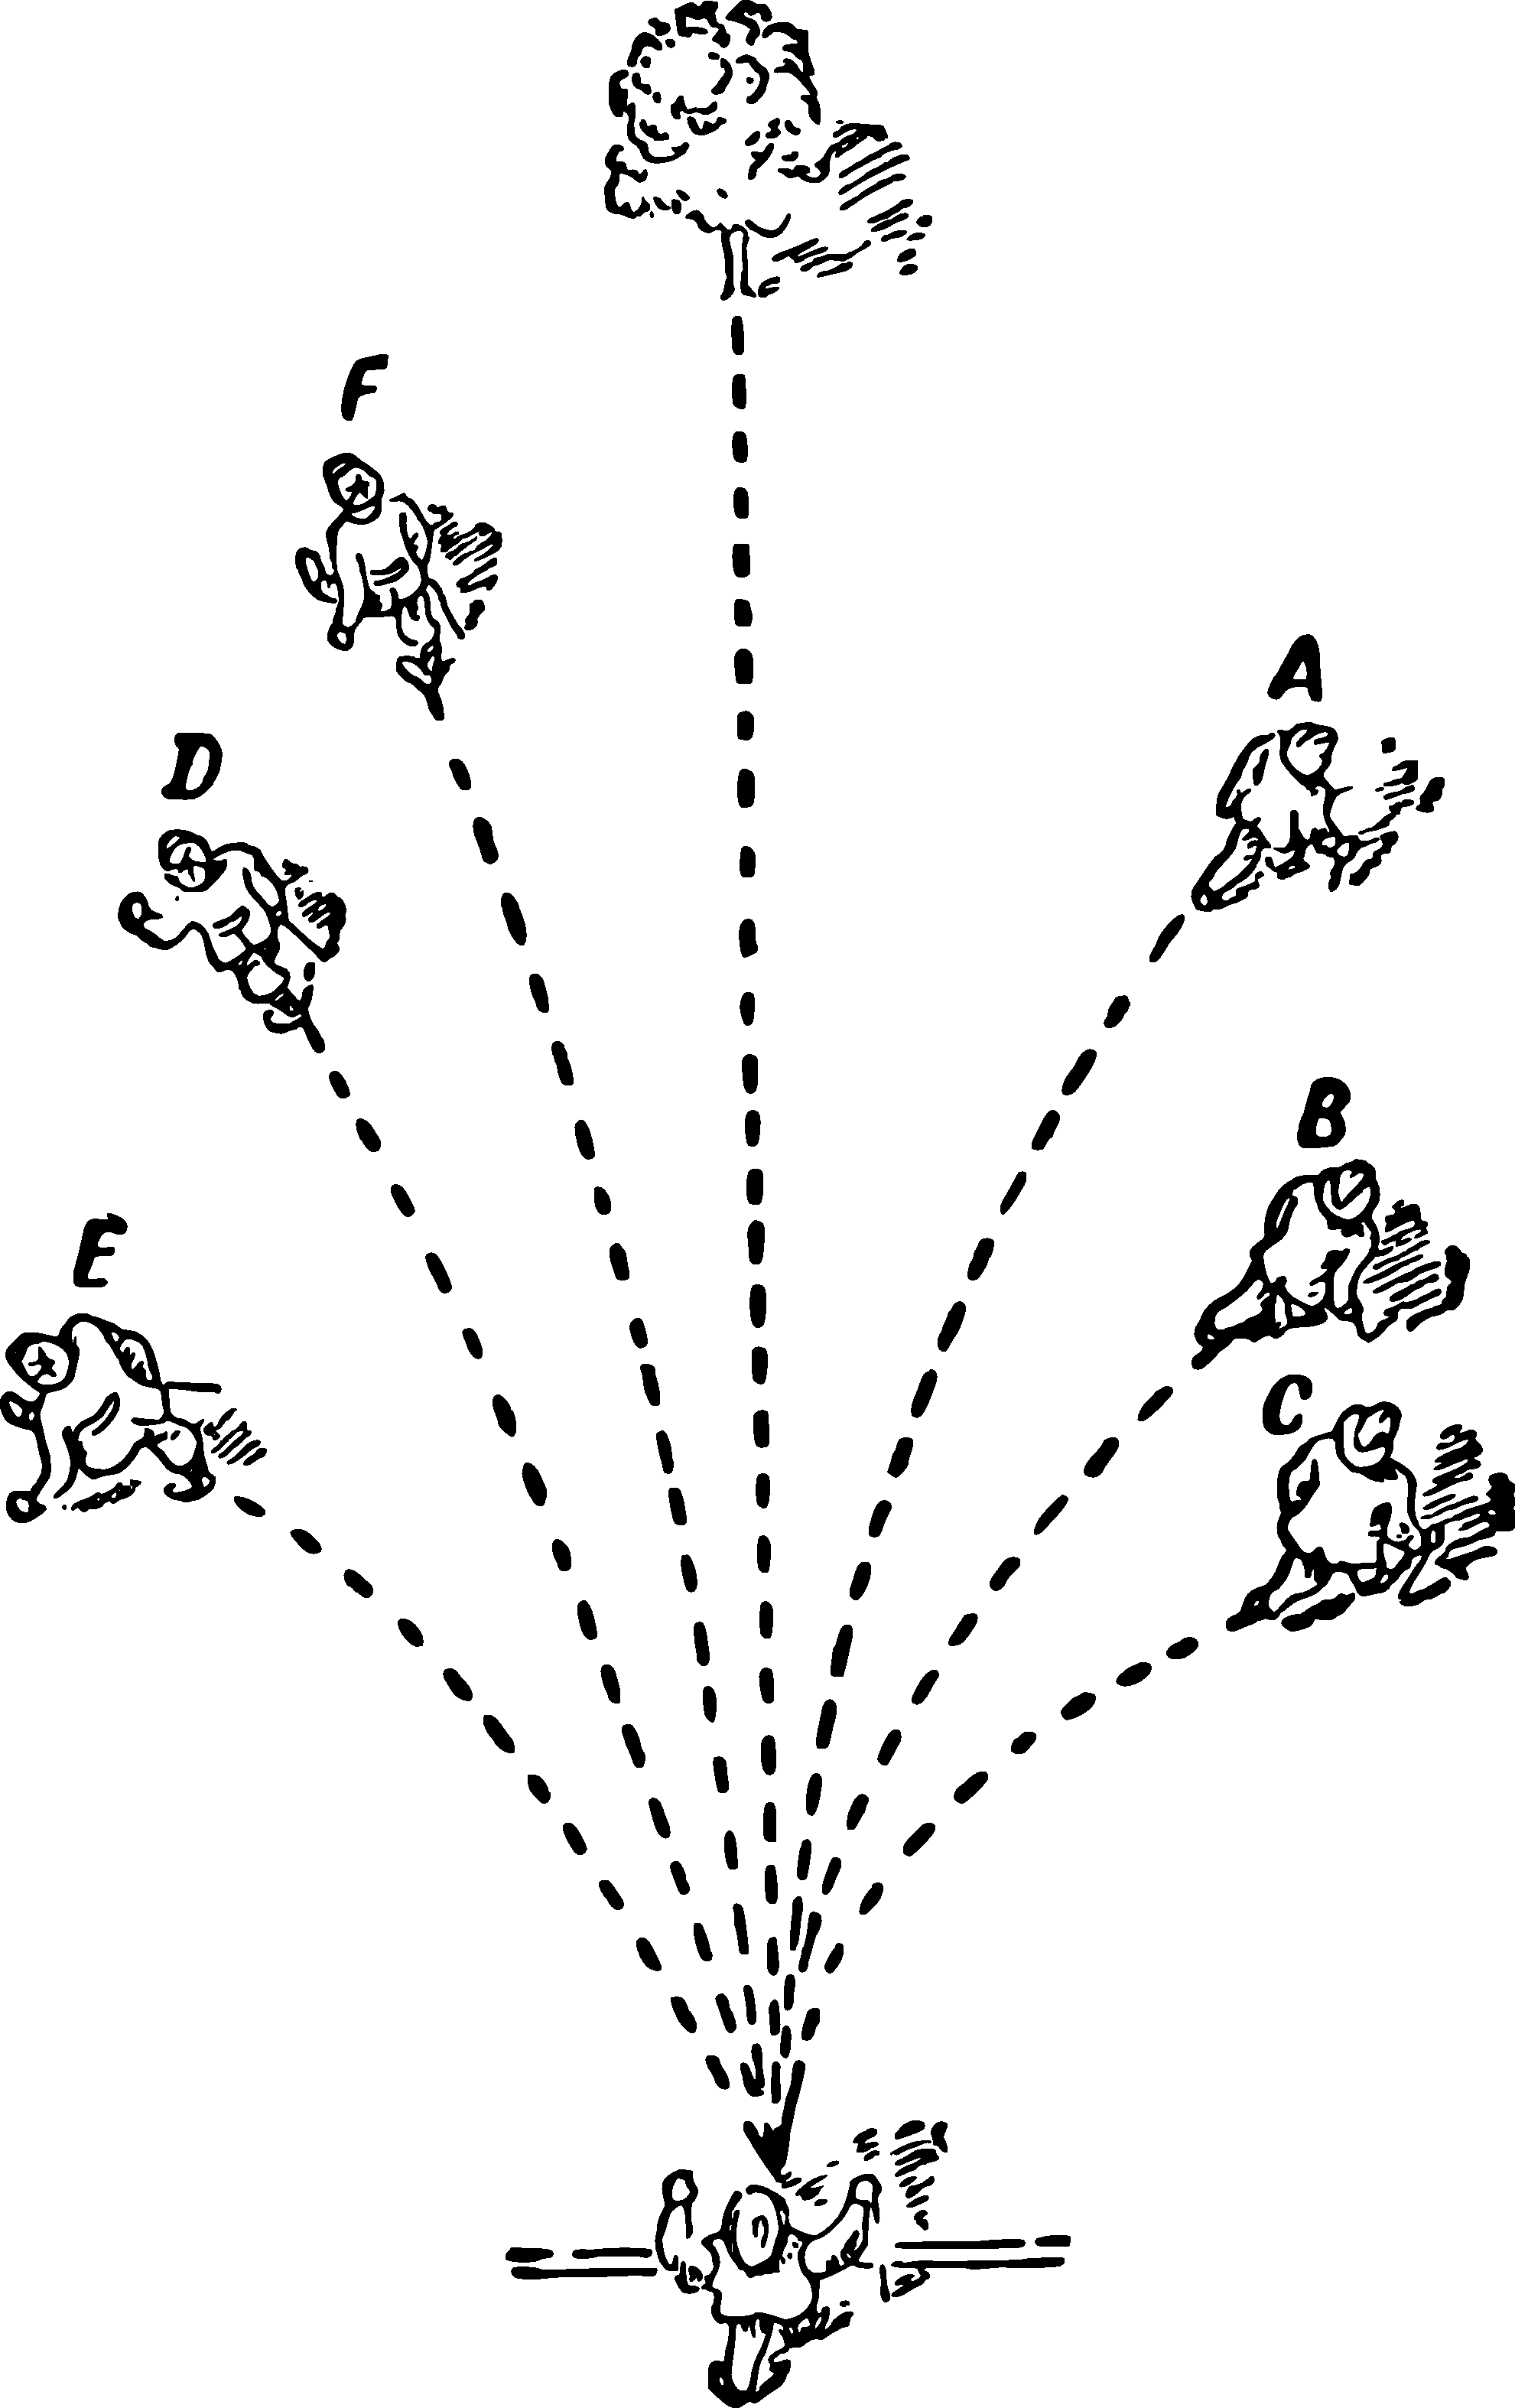
\includegraphics[width=0.65\textwidth]{figures/ch-08/fig-111.pdf}
\sidecaption{Walking with your eyes closed.\label{fig-111}}
\end{figure}

It has long been noticed that travellers wandering without a compass in the desert, across the steppe in a blizzard, or in foggy weather—generally in all cases where there is no opportunity to orient themselves—deviate from the straight path and wander in circles, repeatedly returning to the same place. The radius of the circle described by the pedestrian is about 60–100 meters; the faster the walking, the smaller the radius of the circle, i.e., the tighter the circles closed.

Special experiments have even been conducted to study people's tendency to deviate from a straight path to a circular one. Here's what Hero of the Soviet Union I. Spirin reports on such experiments:
\begin{quote}
On a smooth green aerodrome, a hundred future pilots were lined up. Blindfolds were placed on all of them, and they were instructed to walk straight ahead. The people started walking\dots{} At first, they walked straight; then some started veering to the right, others to the left, gradually began to make circles, returning to their old tracks.
\end{quote}

A similar experiment is known in Venice in St. Mark's Square. People were blindfolded, placed at one end of the square, directly opposite the cathedral, and asked to reach it. Although they only had to walk a mere 175 meters, none of the subjects reached the facade of the building (which is 82 meters wide), and all veered to the side, describing an arc and bumping into one of the 60 stone colonnades (see \figr{fig-112}).


\begin{figure}[h!]
\centering
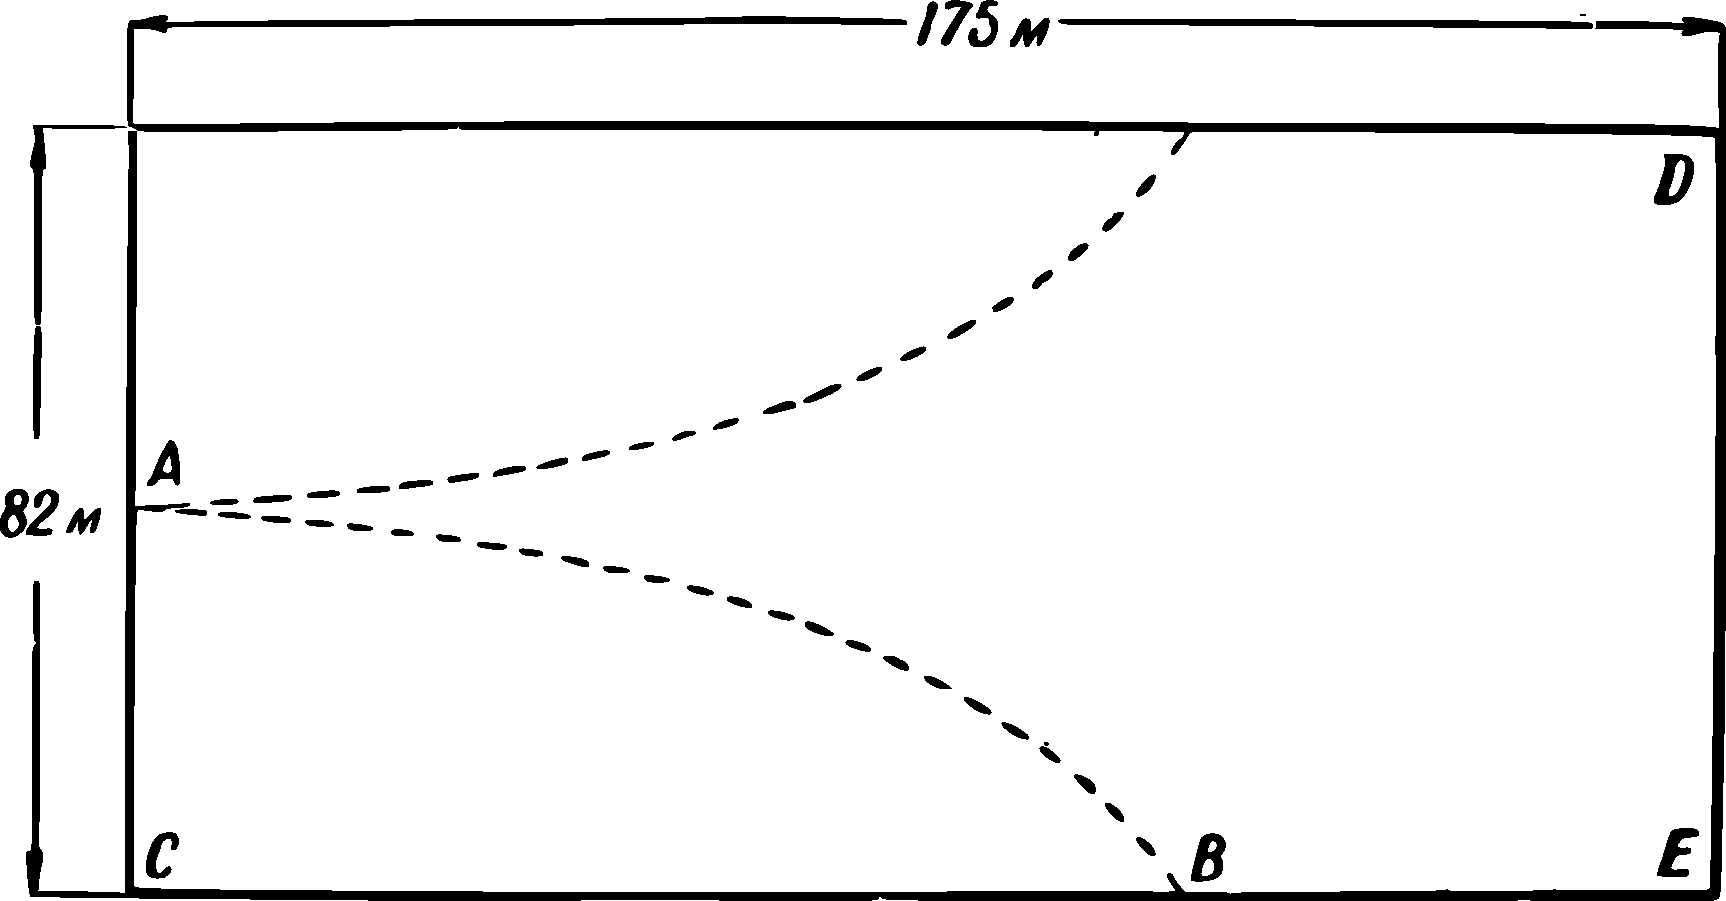
\includegraphics[width=0.9\textwidth]{figures/ch-08/fig-112.pdf}
\sidecaption[][-1cm]{The schematic depiction of the experiment at St. Mark's Square in Venice.\label{fig-112}}
\end{figure}


Anyone who has read Jules Verne's novel \emph{The Adventures of Captain Hatteras} probably remembers the episode where the travellers stumbled upon someone's tracks in a snowy uninhabited desert:
\begin{quote}
`Those are our tracks, my friends!' exclaimed the doctor. `We got lost in the fog and stumbled upon our own tracks \dots{}'
\end{quote}
A classic description of such circular wandering was given to us by Leo Tolstoy in \emph{Master and Man}:
\begin{quote}
Vasiliy Andreyich urged the horse towards where he, for some reason, assumed there was a forest and a watchtower. The snow blinded him, and the wind seemed to want to stop him, but he, leaning forward, continued to drive the horse forward without stopping.

For about five minutes he rode, as it seemed to him, straight ahead, seeing nothing except the horse's head and the white desert.

Suddenly something darkened before him. His heart joyfully pounded, and he rode towards this blackness, already seeing in it the walls of village houses. But black? It turned out to be a tall thistle grown on the boundary\dots{} And for some reason, the sight of this thistle, tormented by the merciless wind, made Vasily Andreyich shudder, and he hastily began to drive the horse, not noticing that, as he approached the thistle, he completely changed his previous direction.

Again something darkened ahead of him. It was another boundary, overgrown with thistle. The dry grass was also desperately thrashed by the wind. Beside it was a horse's hoof print, blown by the wind. Vasily Andreyich stopped, leaned over, looked closely: it was a slightly blown horse's print and could be no one else's but his own. He was evidently circling in a small space.
\end{quote}

Norwegian physiologist Guldborg, who dedicated a special study to wandering (1896), collected a number of carefully verified testimonies about genuine cases of this kind. Let's cite two examples.

\begin{marginfigure}%[h!]
\centering
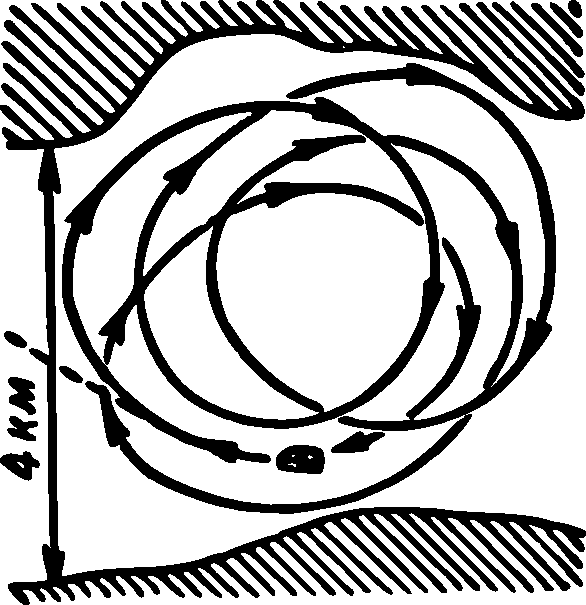
\includegraphics[width=0.8\textwidth]{figures/ch-08/fig-113.pdf}
\sidecaption{The schematic depiction of the wanderings of three travelers.\label{fig-113}}
\end{marginfigure}


Three travellers intended to leave the guard post on a snowy night and exit the valley, which was 4 km wide, to reach their home, located in the direction indicated by the dashed line on the attached diagram (\figr{fig-113}). Along the way, they imperceptibly veered to the right, following the curve marked by the arrow. After covering some distance, they, according to their calculations, believed they had reached their destination -- when in fact they found themselves back at the same guard post they had left. Setting out on the path again, they veered even further off course and again arrived at the starting point. The same thing happened for the third and fourth times. In desperation, they made a fifth attempt -- but with the same result. After the fifth round, they gave up further attempts to leave the valley and waited for morning.

\begin{figure}[h!]
\centering
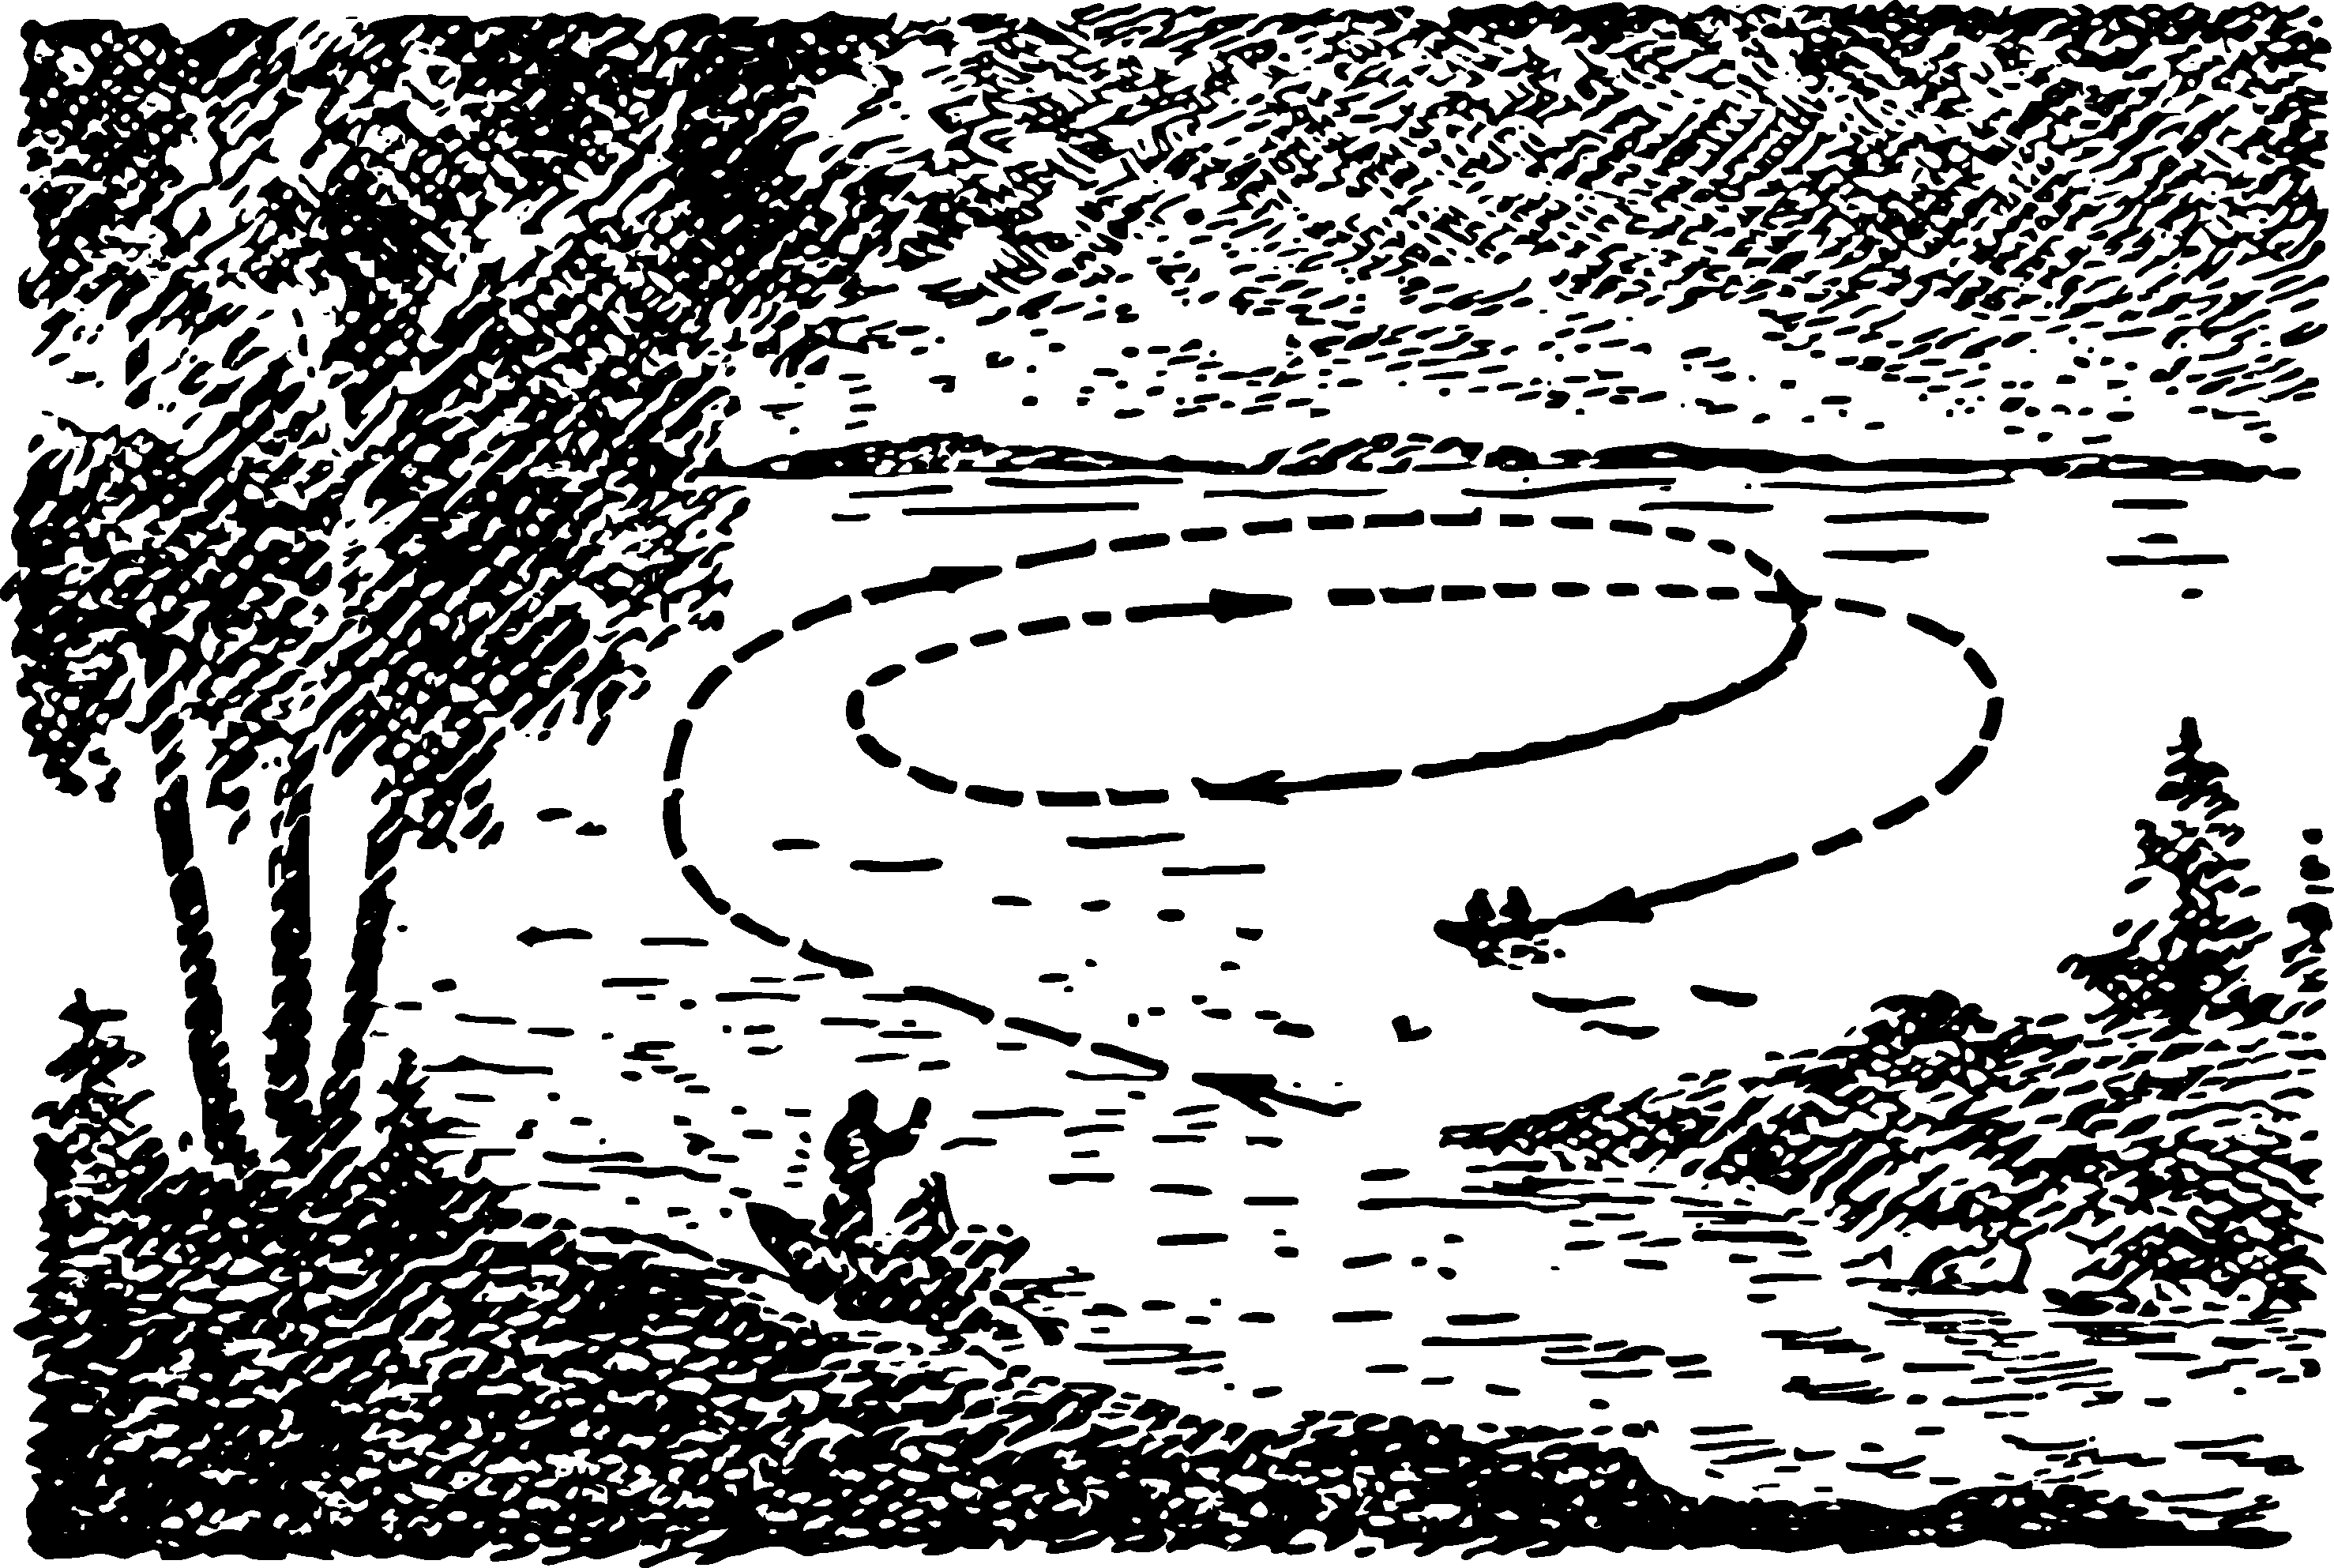
\includegraphics[width=0.9\textwidth]{figures/ch-08/fig-114.pdf}
\sidecaption{How the rowers attempted to cross the strait in foggy weather.\label{fig-114}}
\end{figure}


Even more difficult is rowing straight on the sea in a dark, starless night or in thick fog. There is a case, one of many similar ones, when rowers, intending to cross a strait 4 miles wide in foggy weather, twice ended up on the opposite shore, but did not reach it, and unconsciously circled twice before finally\dots{} landing back at their point of departure (\figr{fig-114}).

The same happens with animals. Polar travellers tell of circles drawn in the snow deserts by animals harnessed to sleds. Dogs, allowed to swim with their eyes blindfolded, also describe circles in the water. Blinded birds also fly in circles. A frightened animal, deprived of the ability to orient itself from fear, does not save itself in a straight line but in a spiral.

Zoologists have found that tadpoles, crabs, jellyfish, even microscopic amoebas in a drop of water all move in a circle.

What explains the mysterious preference of humans and animals for circles, the inability to maintain a straight direction in the dark? The question will immediately lose its seeming mystery in our eyes if we put it correctly.

Let's not ask why animals move in circles, but what they need to move in a straight line? Think about how a wind-up toy cart moves. Sometimes the cart doesn't roll straight but veers to the side. In this curved movement, no one sees anything mysterious; everyone guesses why this happens: obviously, the right wheels are not equal to the left ones.

It's clear that a living creature can only move in a straight line without the help of eyes if the muscles on its right and left sides work exactly the same. But the point is that the symmetry of the human and animal body is incomplete. In the vast majority of people and animals, the muscles on the right side of the body are not equally developed as the muscles on the left. Naturally, a pedestrian who always steps a little further with his right leg than his left will not be able to keep a straight line; if his eyes don't help him correct his path, he will inevitably veer to the left. Similarly, a rower, when deprived of the ability to orient himself due to fog, will inevitably veer to the left if his right arm works stronger than his left. This is a geometric necessity.

Imagine, for example, that when lifting the left leg, a person takes a step one millimetre longer than with the right leg. Then, by alternating each leg for a thousand steps, the person will describe a path with the left leg that is \SI{1000}{\milli\meter}, or a whole meter, longer than with the right leg. This is impossible on straight parallel paths, but quite feasible on concentric circles.
\begin{figure}[h!]
\centering
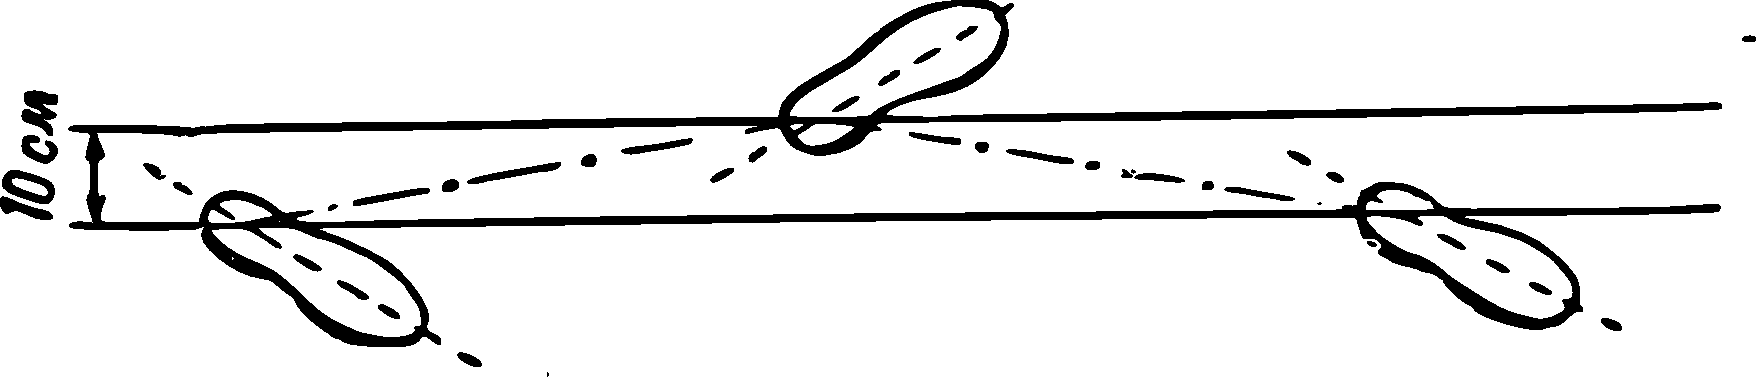
\includegraphics[width=0.9\textwidth]{figures/ch-08/fig-115.pdf}
\sidecaption{The lines of the prints of the right and left feet when walking.\label{fig-115}}
\end{figure}


We can even, using the plan of the circular movement described above in the snowy valley, calculate how much longer the step of those travellers was with the left leg compared to the right (since the path curved to the right, it is clear that it was the left leg that took longer steps). The distance between the lines of imprints of the right and left legs during walking (see \figr{fig-115}) is approximately \SI{10}{\centi\meter}, or \SI{0.1}{\meter}. When a person completes one full circle, their right leg covers a distance of $2\pi R$, and the left leg covers $2\pi(R + 0.1)$, where $R$ is the radius of this circle in meters. 



The difference is $2\pi(R + 0.1) - 2 \pi R  = 2 \pi(0.1)$, which equals \SI{0.62}{\meter}, or \SI{620}{\milli\meter}, due to the difference in length between the left and right steps, repeated as many times as steps were taken. From \figr{fig-113}, we can deduce that our travellers described circles with a diameter of approximately \SI{3.5}{\kilo\meter}, or a length of about \SI{10000}{\meter}. With an average step length of \SI{0.7}{\meter} over a distance of \SI{10000}{\meter}, this equals $10000/0.7 = 14000$ steps; of these, 7000 were with the right leg and the same with the left. Thus, we find that 7000 ``left'' steps exceeded 7000 ``right'' steps by \SI{620}{\milli\meter}.

Hence, one left step is longer than one right step by 620/7000 mm, or less than \SI{0.1}{\milli\meter}. Here's how such a tiny difference in steps can result in such a striking outcome!

The radius of the circle that the wanderer describes depends on the difference in lengths between the ``right'' and ``left'' steps. This dependency is easy to establish. The total number of steps taken over one circle, with a step length of \SI{0.7}{\meter} , is $2\pi R/0.7$, where $R$ is the radius of the circle in meters; of these, there are $2 \pi R/2 \cdot 0.7$ ``left'' steps and the same number of ``right'' steps. Multiplying this number by the magnitude of the difference $x$ in the length of the steps, we obtain the difference in the lengths of those concentric circles that are described by the left and right legs, i.e.:
\begin{equation*}%
\frac{2\pi Rx}{2 \cdot 0.7} = 2\pi \cdot 0.1 \qor Rx = 0.14,
\end{equation*}
where $R$ and $x$ are in meters.

By this simple formula, it is easy to calculate the radius of the circle when the difference in steps is known, and vice versa. For example, for the participants of the experiment in Piazza San Marco in Venice, we can establish the maximum radius of the circles described by them while walking. Indeed, since none of them reached the facade $DE$ of the building (see \figr{fig-112}), then according to the ``arrow'' $AC = \SI{41}{\meter}$ and the chord $BC$, which does not exceed \SI{175}{\meter}, we can calculate the maximum radius of the arc $AB$. It is determined by the equality
\begin{equation*}%
2R = \frac{BC^{2}}{AC} = \frac{175^{2}}{41} = \SI{750}{\meter}, 
\end{equation*}
from which $R$, the maximum radius, will be about \SI{370}{\meter}. 

Knowing this, we determine the minimum value of the difference in step lengths from the formula obtained earlier:
\begin{equation*}%
370 x = 0.14, \,\, \text{hence}\,\, x = \SI{0.4}{\milli\meter}.
\end{equation*}
Sometimes you have to read and hear that the fact of circling while walking blindly depends on the difference in length between the right and left legs; since the left leg is longer for most people, they must inevitably deviate to the right from the straight direction while walking. Such an explanation is based on a geometric error. The important factor is the difference in step lengths, not leg lengths. From \figr{fig-116}, it is clear that even with a difference in leg length, one can still make strictly identical steps if each leg is extended at the same angle while walking, i.e., stepping so that $\angle B_{1} = \angle B$. Since in this case always $A_{1}B_{1} = AB$ and $B_{1}C_{1} = BC$, then $\triangle A_{1}B_{1}C_{1} \cong \triangle ABC$, and therefore $AC = C_{1}A_{1}$. Conversely, with strictly identical leg lengths, steps can be of different lengths if one leg is extended farther while walking than the other.
\begin{figure}[h!]
\centering
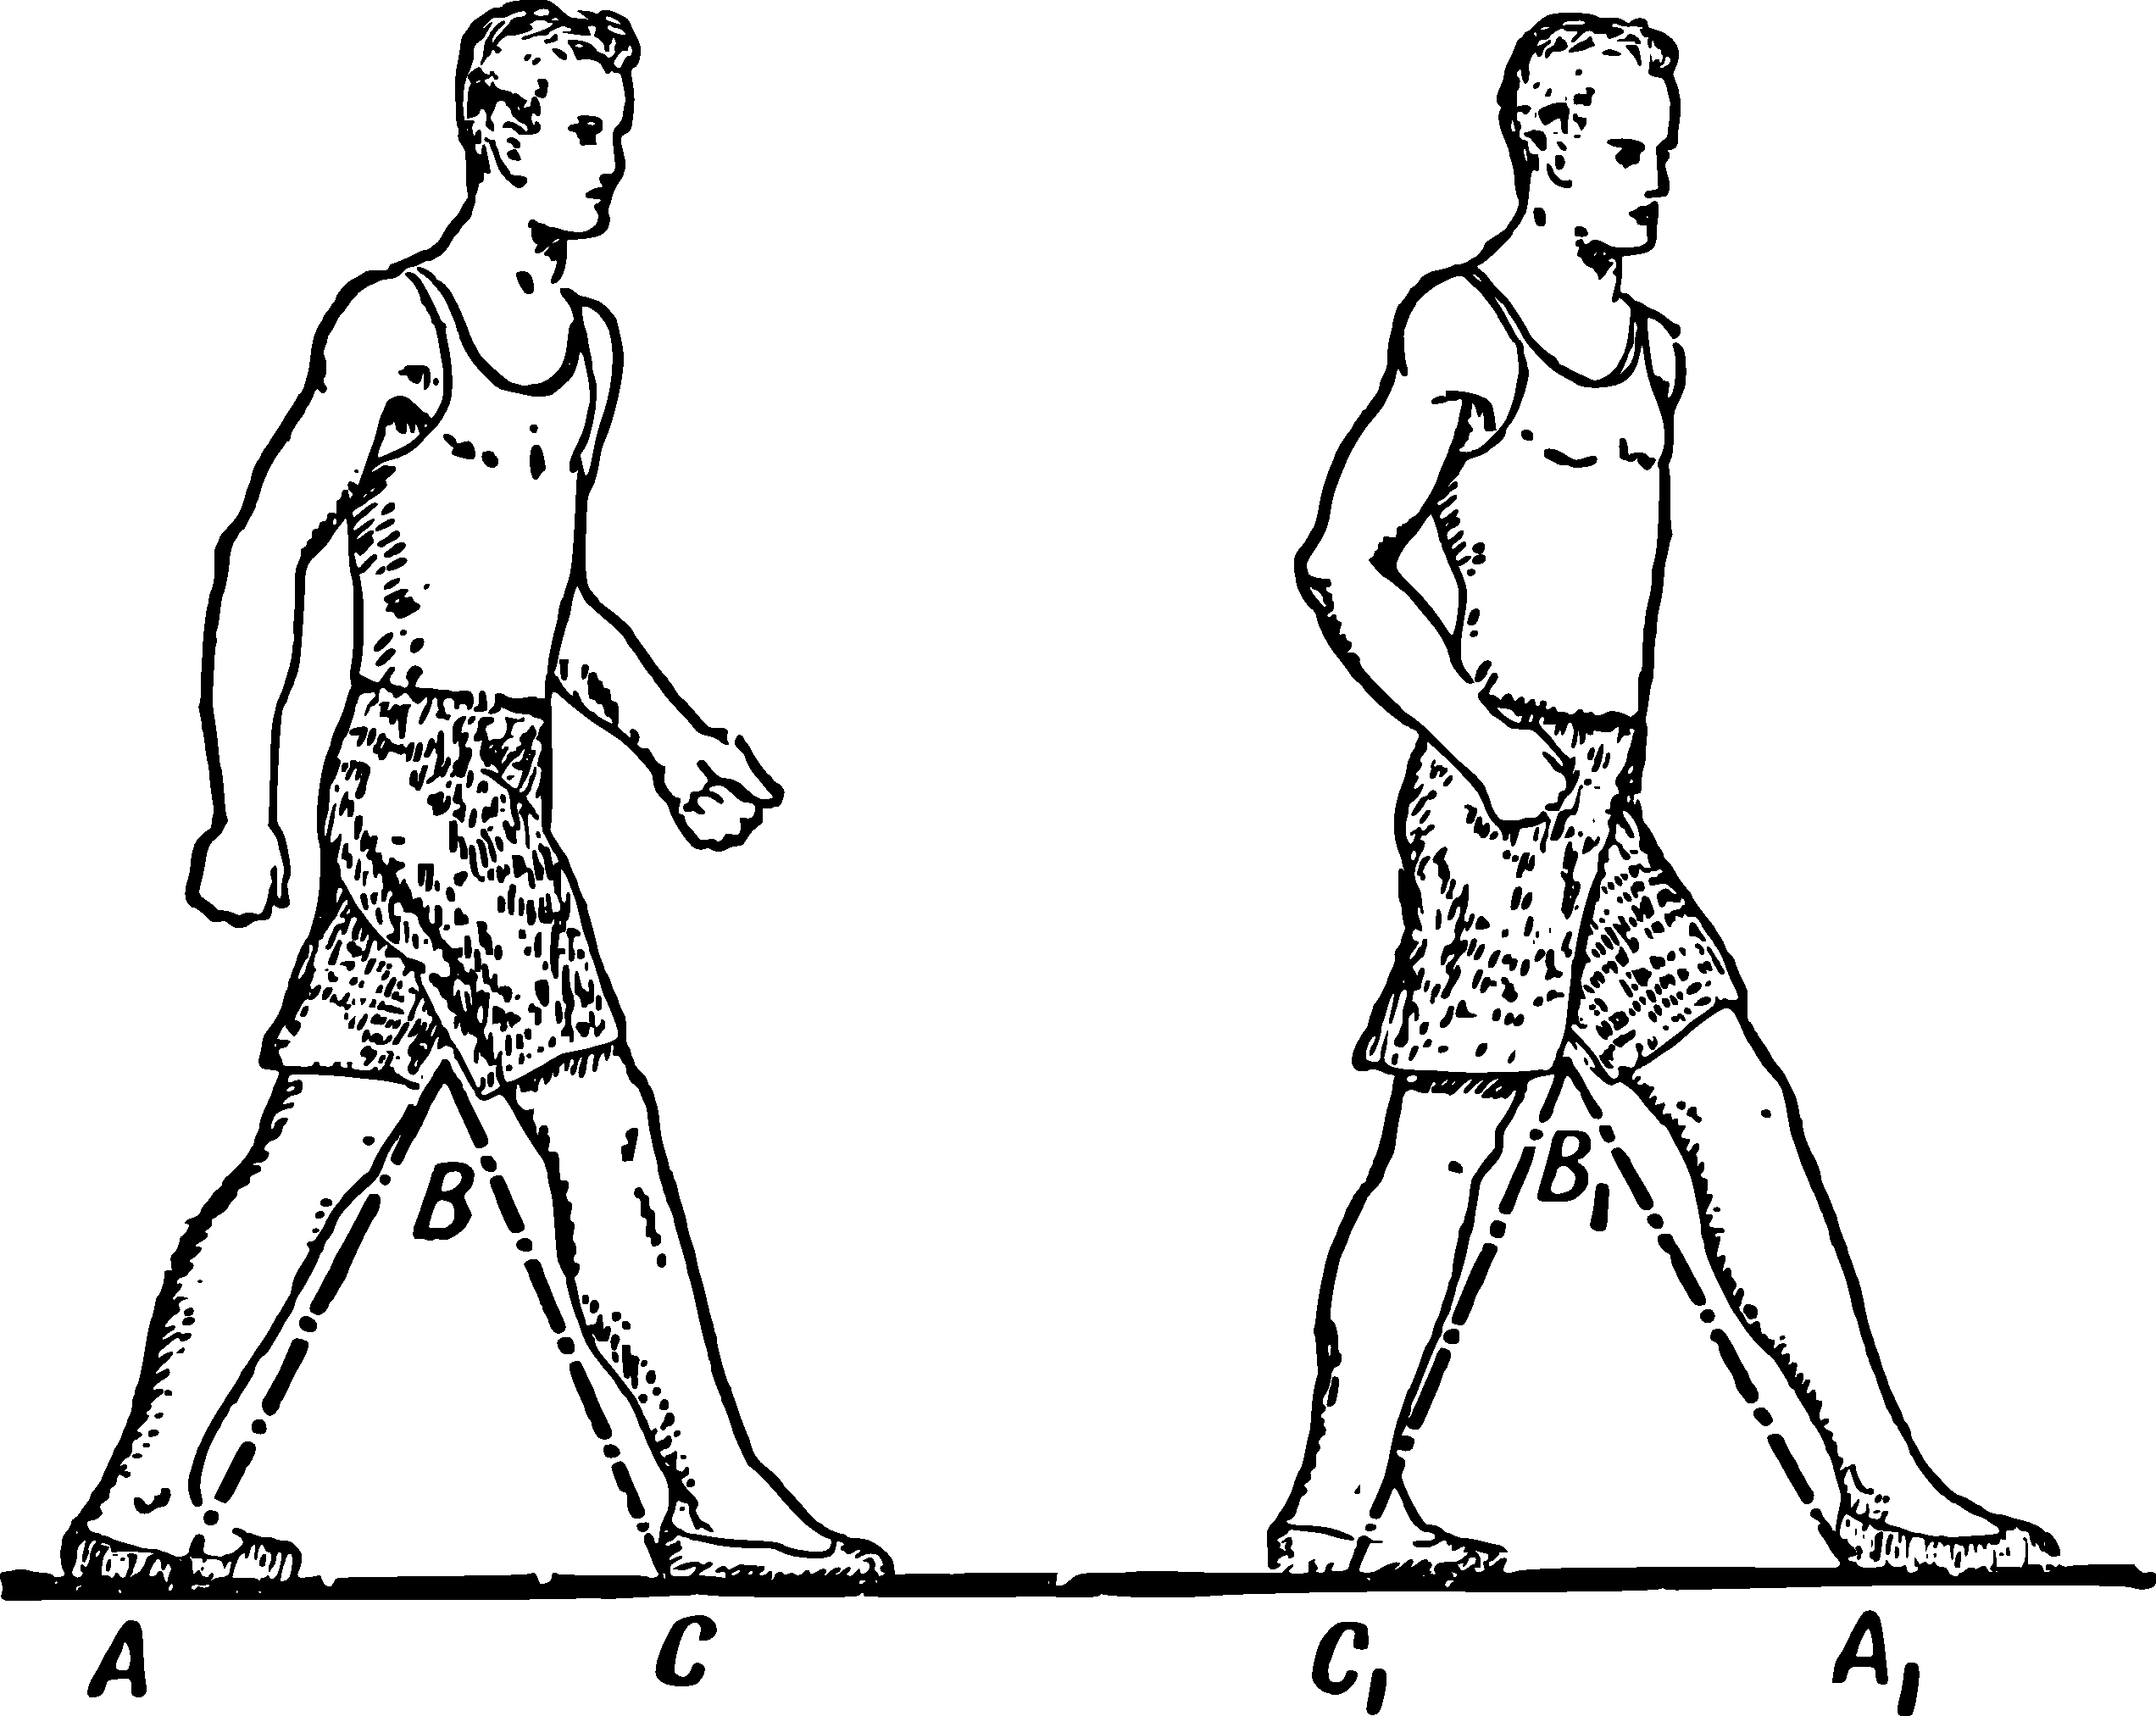
\includegraphics[width=0.8\textwidth]{figures/ch-08/fig-116.pdf}
\sidecaption{If the angle of each step is the same, then the steps will be exactly the same.\label{fig-116}}
\end{figure}

For a similar reason, a boatman rowing stronger with his right hand than with his left must inevitably lead the boat in a circle, bending to the left. Animals making uneven steps with their right or left legs, or birds making unequal strokes with their right and left wings, must also move in circles whenever they are unable to control straight-line direction with sight. Here too, a very slight difference in the strength of the arms, legs, or wings is sufficient.

With this perspective, the mentioned phenomena lose their mystery and become entirely natural. It would be astonishing if people and animals, on the contrary, could maintain a straight direction without controlling it with their eyes. After all, a necessary condition for this is strict geometric symmetry of the body, absolutely impossible for living organisms. The slightest deviation from mathematically perfect symmetry must inevitably result in circling. The miracle is not what we marvel at here but rather that we were willing to consider it natural.

The inability to maintain a straight path is not a significant obstacle for humans: compasses, roads, and maps save them in most cases from the consequences of this deficiency.

For animals, especially those inhabiting deserts, steppes, and vast expanses of the sea, the asymmetry of their bodies, which compels them to describe circles instead of straight lines, is an important factor in their lives. It's as if an invisible chain binds them to their birthplace, depriving them of the ability to move away from it significantly. The gazelle, daring to venture far into the desert, inevitably returns back. Seagulls, leaving their native cliffs to fly into the open sea, cannot help but return to their nests (which makes the long flights of birds that cross continents and oceans in a straight direction all the more mysterious).


\section{Measuring with Bare Hands}
\label{sec-8.8}

The boy from Mayne-Reid's story was able to solve his geometric problem successfully only because he had measured his height shortly before the journey and remembered the measurement results. It would be beneficial for each of us to have such a `living meter' so that we could use it for measurements when needed. It is also useful to remember that for most people, the distance between the ends of their outstretched arms is equal to their height (see \figr{fig-117}) -- a fact marked by the ingenious artist and scientist Leonardo da Vinci; this makes it more convenient to use our `living meters' than what the boy did in Mayne-Reid's story. 

On average, the height of an adult (of Slavic descent) is about 1.7 meters, or 170 centimeters: this is easy to remember. However, it is not advisable to rely on the average value: everyone should measure their height and the span of their arms.

\begin{figure}[h!]
\centering
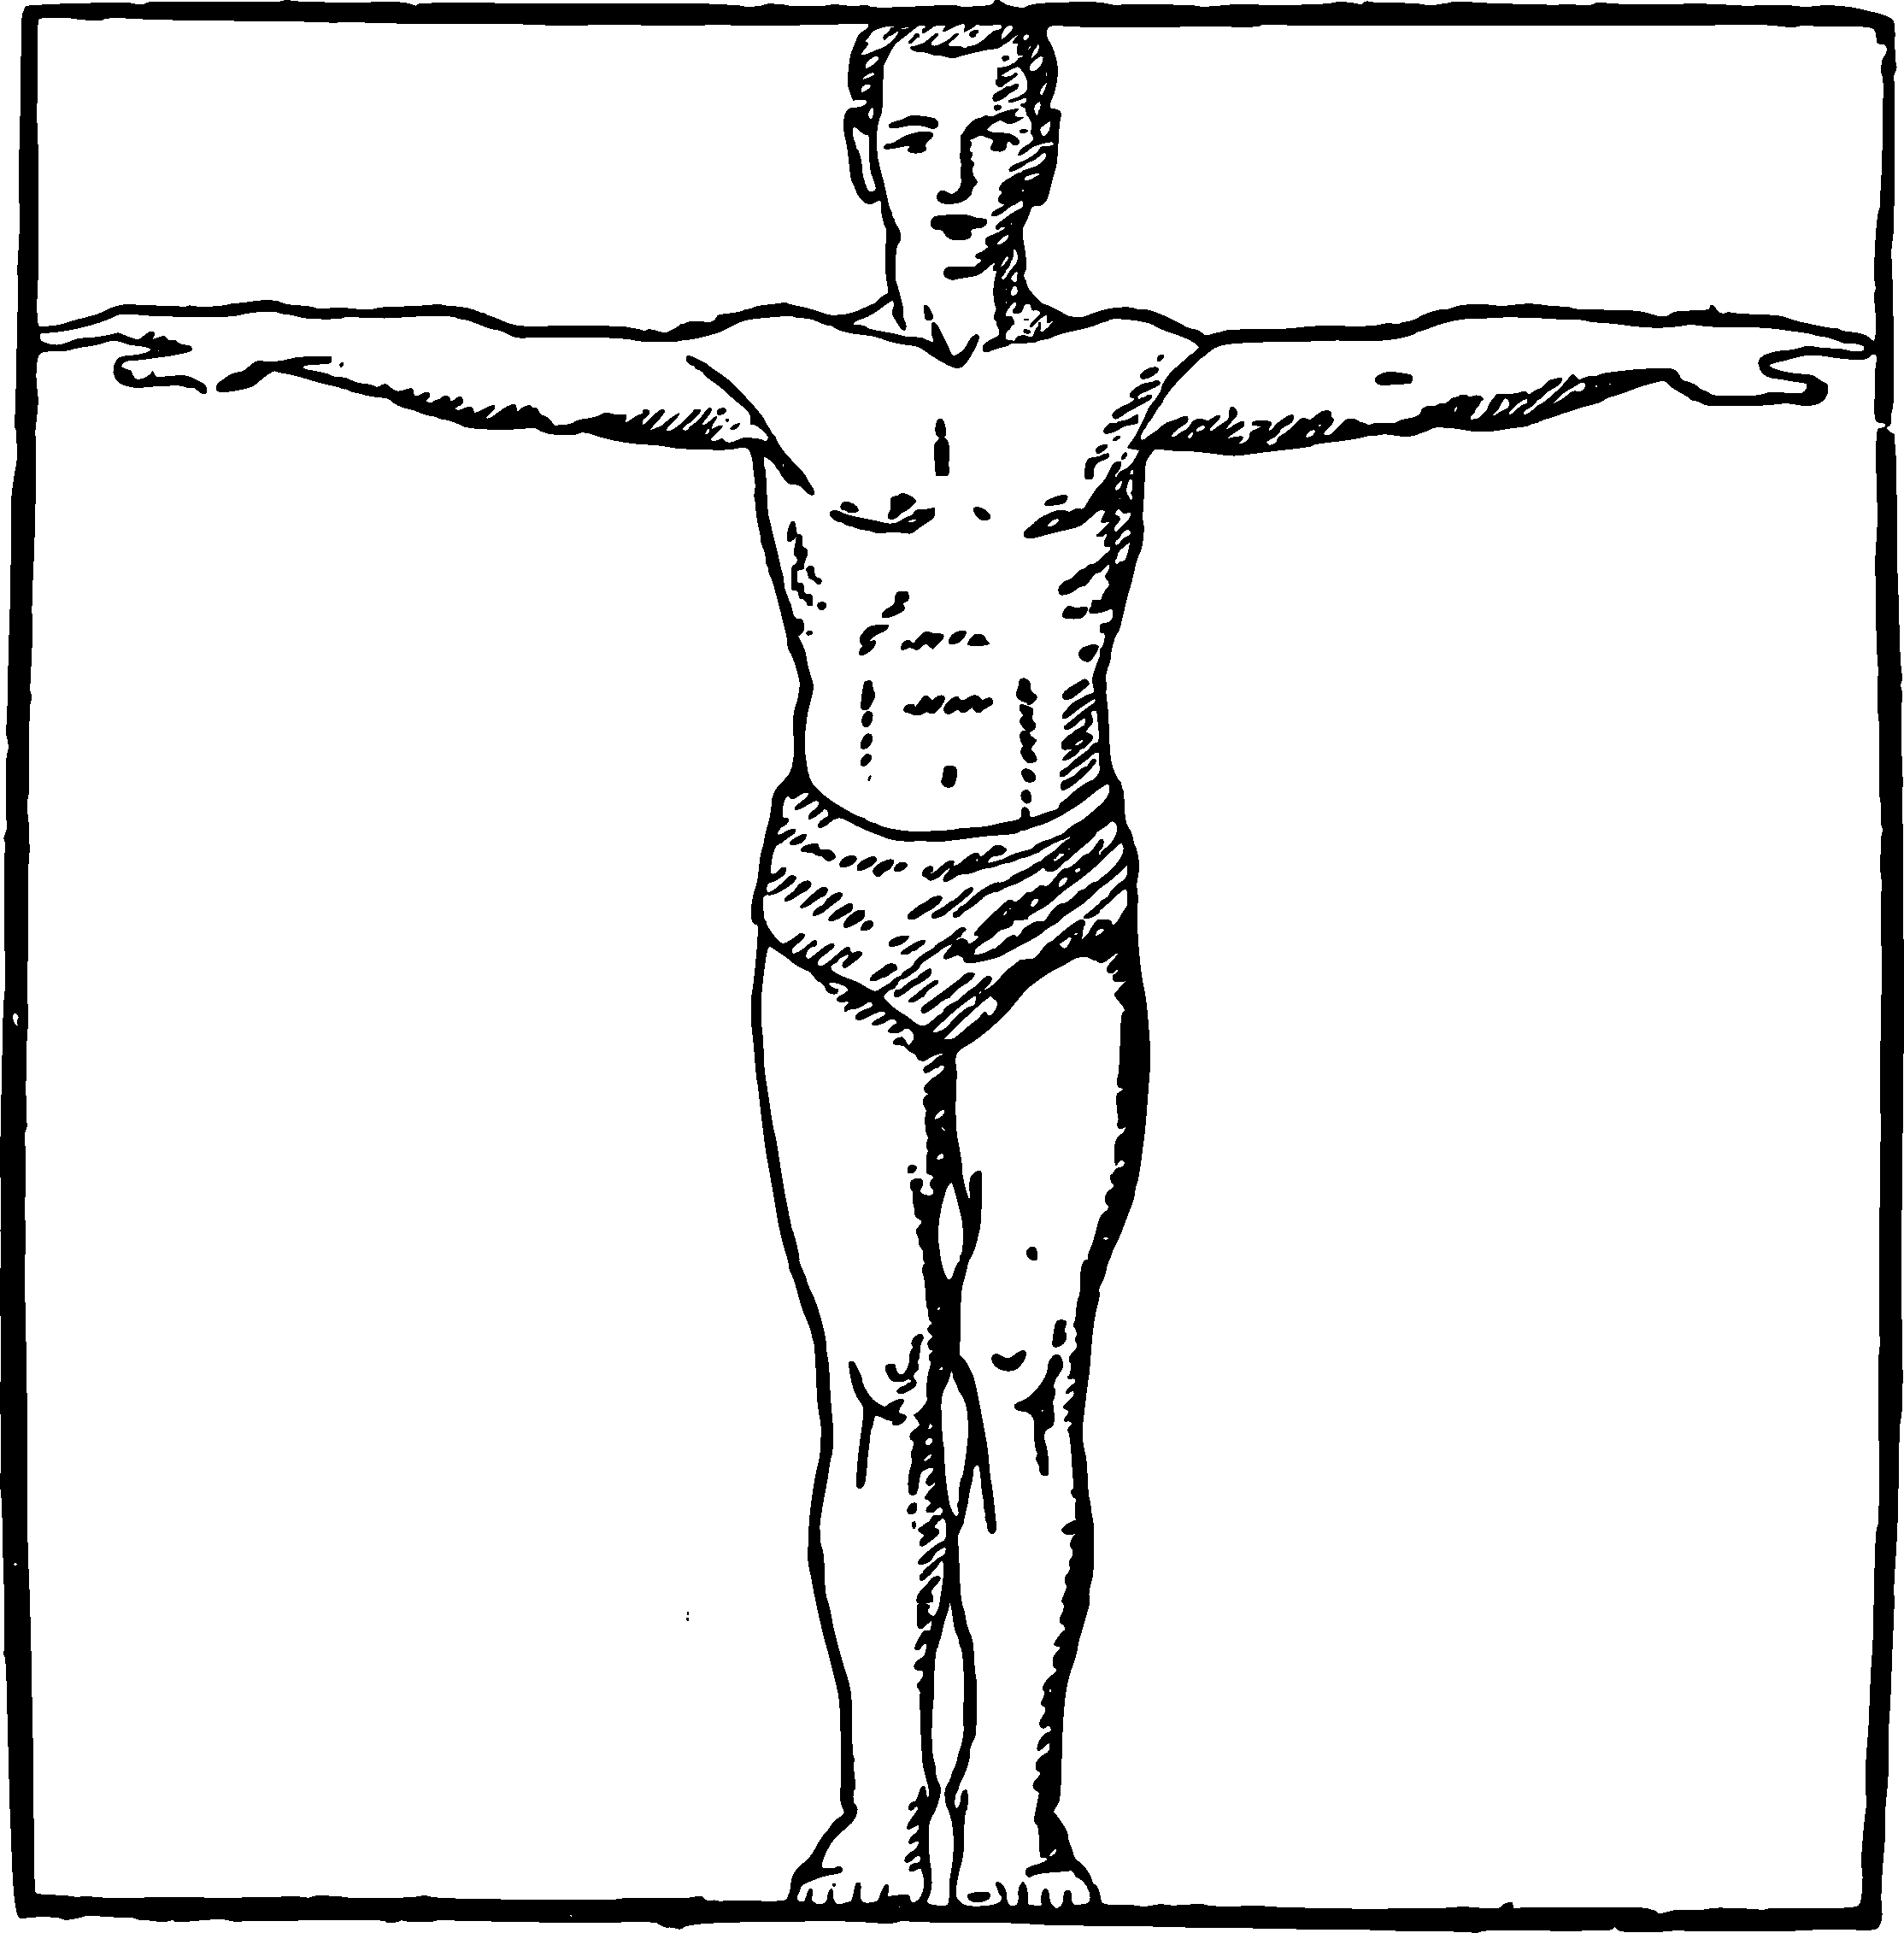
\includegraphics[width=0.8\textwidth]{figures/ch-08/fig-117.pdf}
\sidecaption{The Leonardo da Vinci rule -- the vitruvian man.\label{fig-117}}
\end{figure}

For measuring small distances without a scale, it is useful to remember the length of one's ``quarter'', i.e., the distance between the tips of the thumb and little finger when fully stretched (see \figr{fig-118}). For an adult man, it is about 18 centimetres -- roughly one ``arshin''(hence the name ``quarter''); however, it is smaller in young people and gradually increases with age (up to 25 years).


\begin{figure}[h!]
\centering
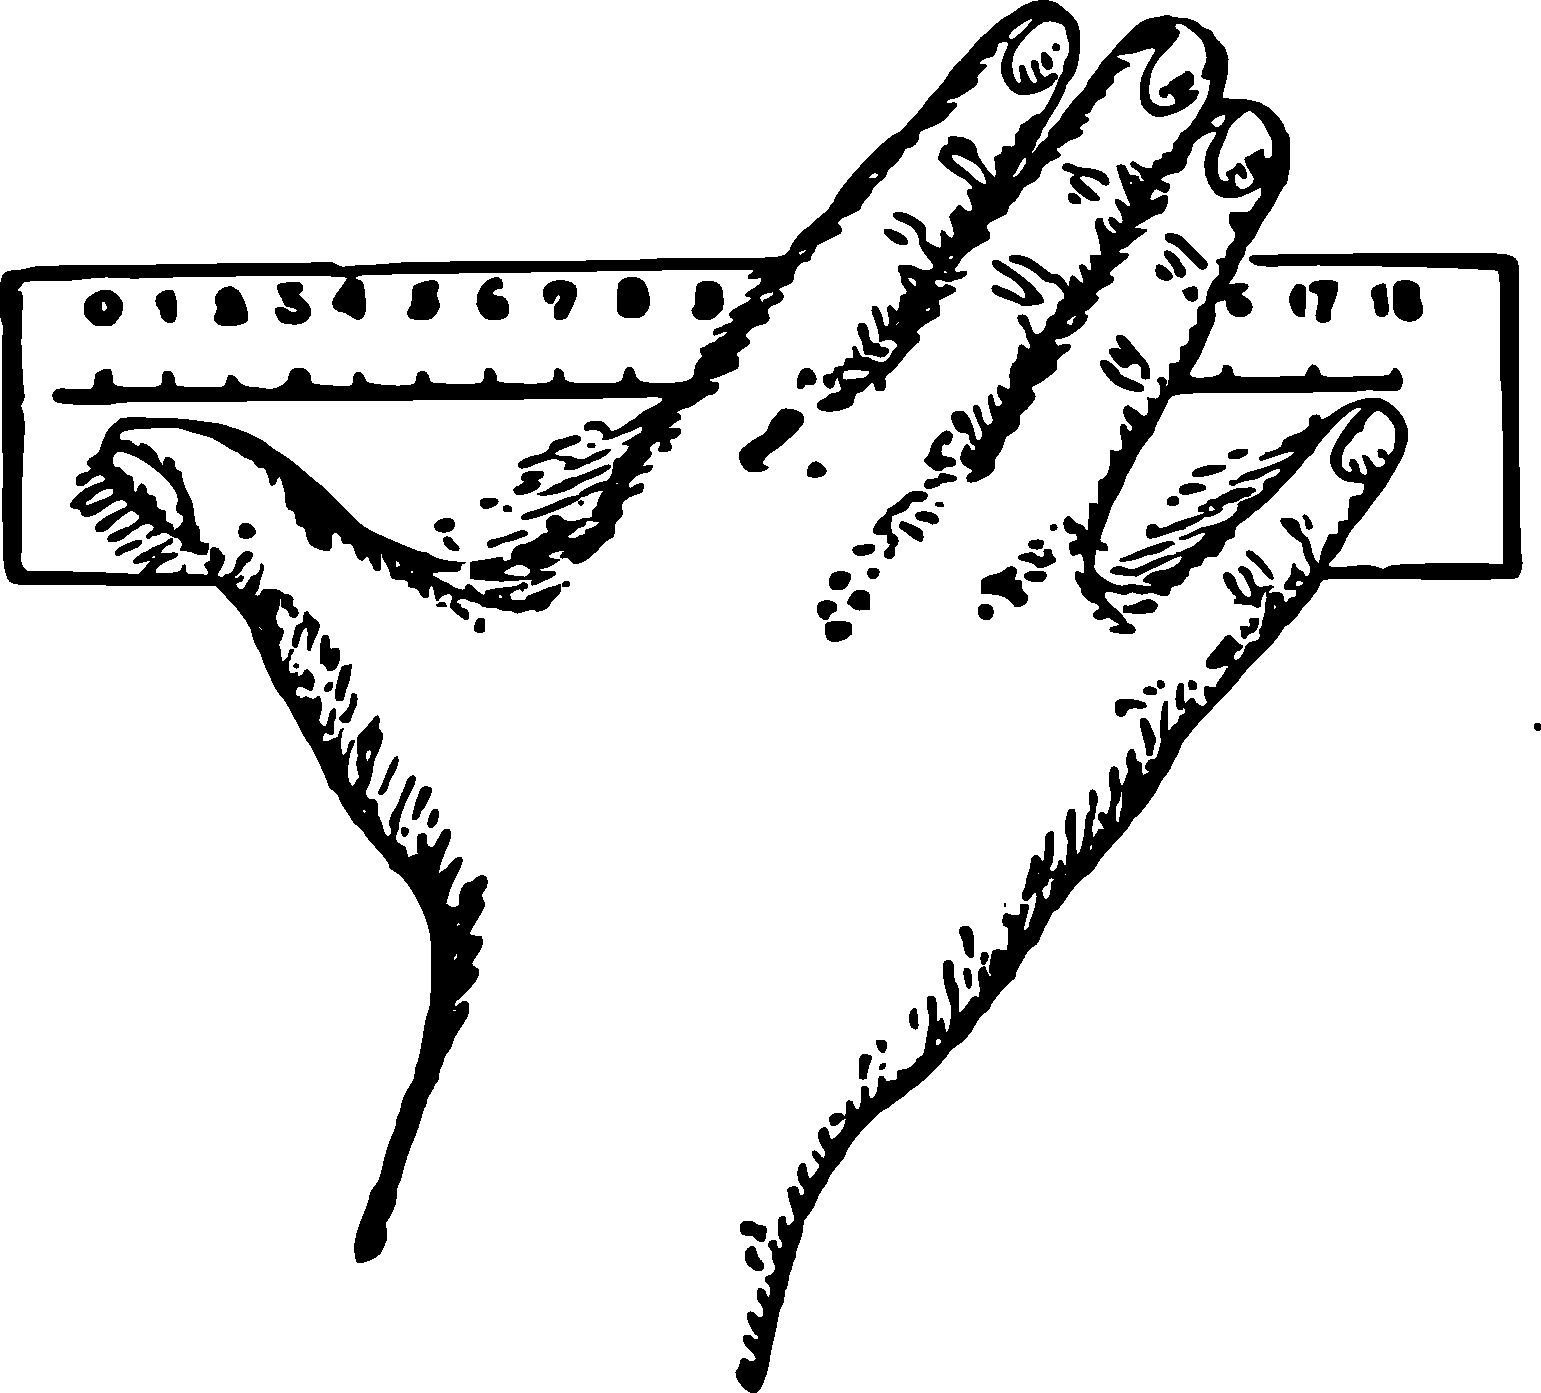
\includegraphics[width=0.4\textwidth]{figures/ch-08/fig-118.pdf}
\sidecaption[][-1cm]{Measuring the distance between the ends of the fingers.\label{fig-118}}
\end{figure}

Furthermore, for the same purpose, it is useful to measure and remember the length of your index finger, considering it in two ways: from the tip to the middle finger (see \figr{fig-119}) and from the base of the thumb.

\begin{figure}[h!]
\centering
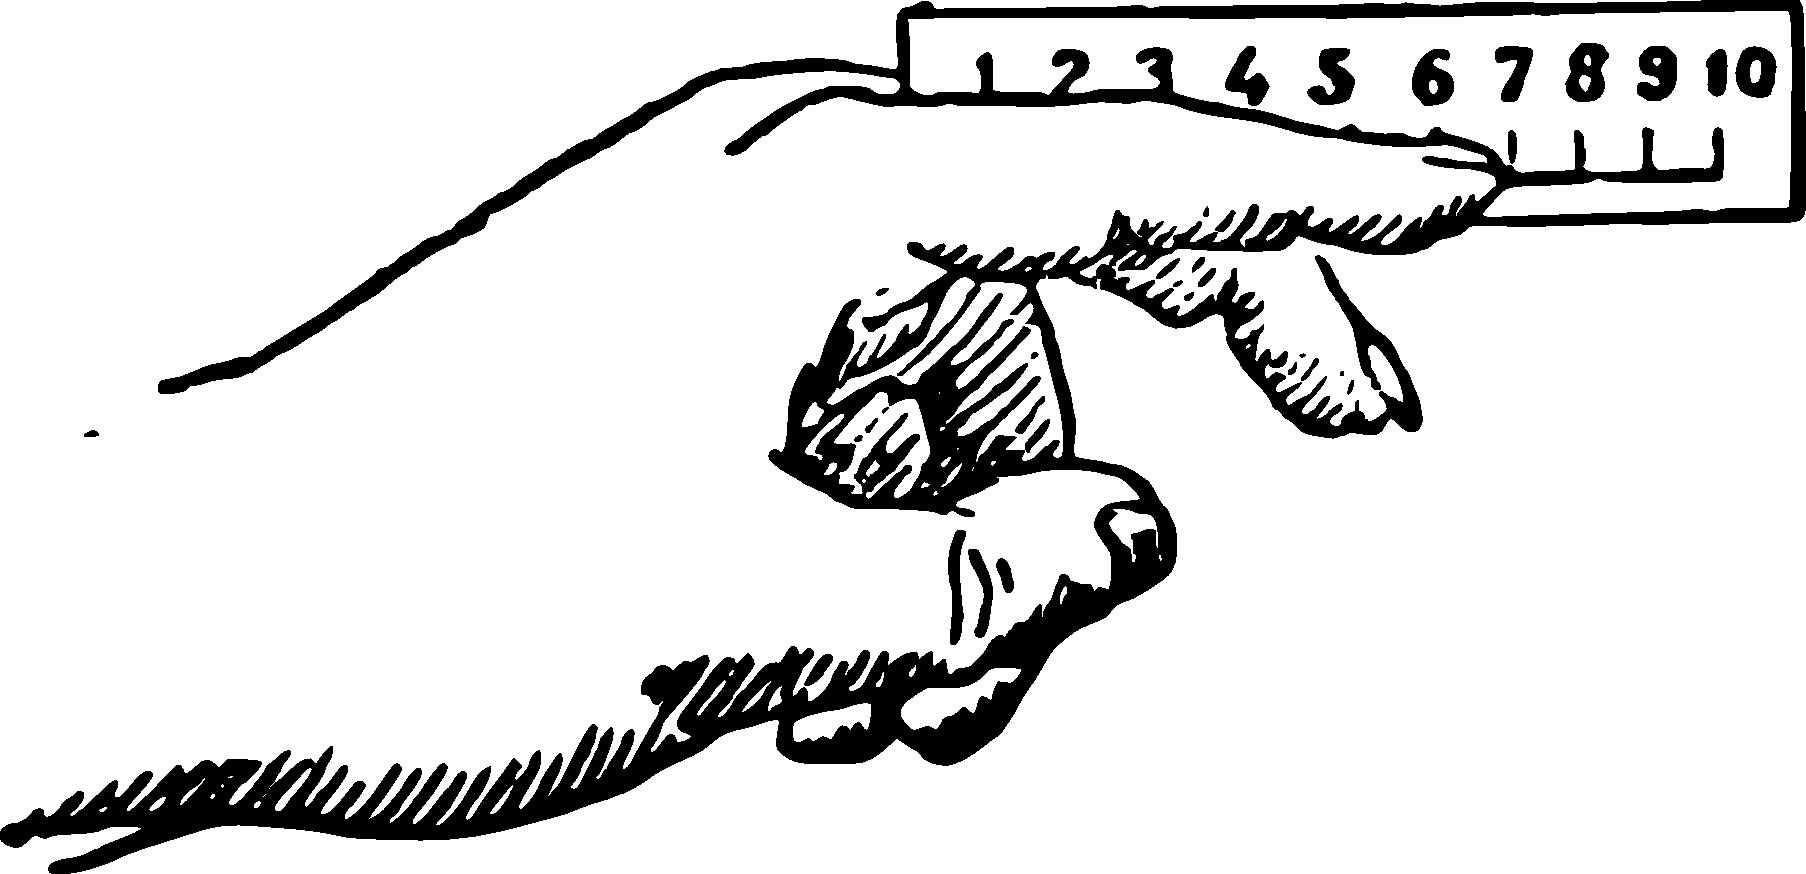
\includegraphics[width=0.5\textwidth]{figures/ch-08/fig-119.pdf}
\sidecaption[][-2cm]{Measuring the length of the index finger.\label{fig-119}}
\end{figure}


Similarly, you should know the maximum distance between the tips of the index and middle fingers, which is about 19 centimeters for an adult (see \figr{fig-120}). Finally, you need to know the width of your fingers. The width of three middle fingers, tightly clenched, is approximately 5 centimeters.

\begin{figure}[h!]
\centering
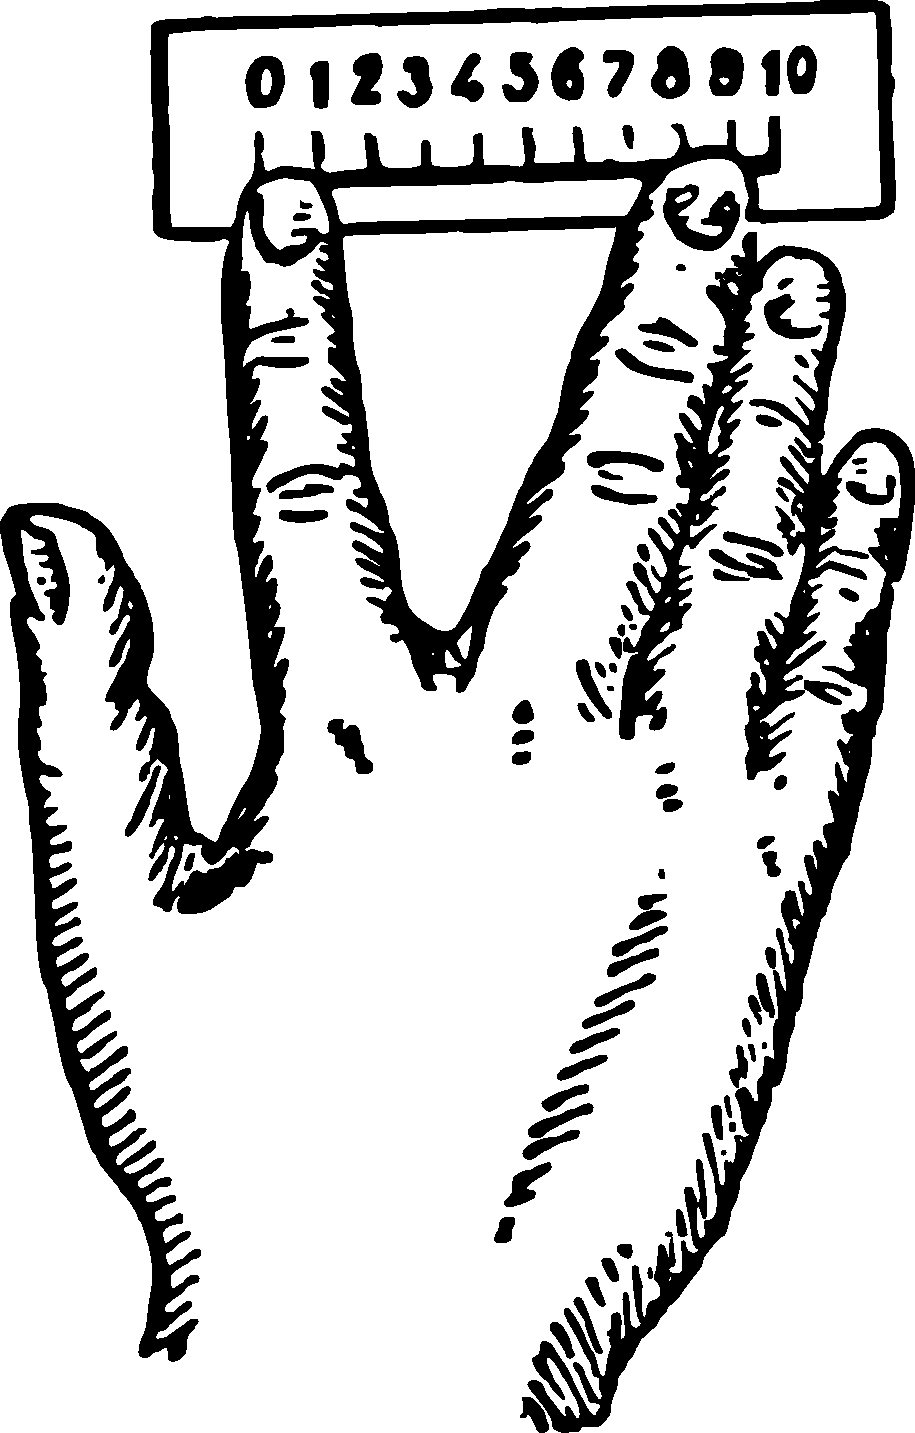
\includegraphics[width=0.25\textwidth]{figures/ch-08/fig-120.pdf}
\sidecaption{Measuring the distance between the ends of two fingers.\label{fig-120}}
\end{figure}


Armed with all this information, you will be able to perform various measurements quite satisfactorily literally with your bare hands, even in the dark. An example is presented in \figr{fig-121}: here, the circumference of a glass is measured using fingers. Based on average values, it can be said that the circumference of the glass is equal to 18 + 5, i.e., 23 centimeters.


\begin{figure}[h!]
\centering
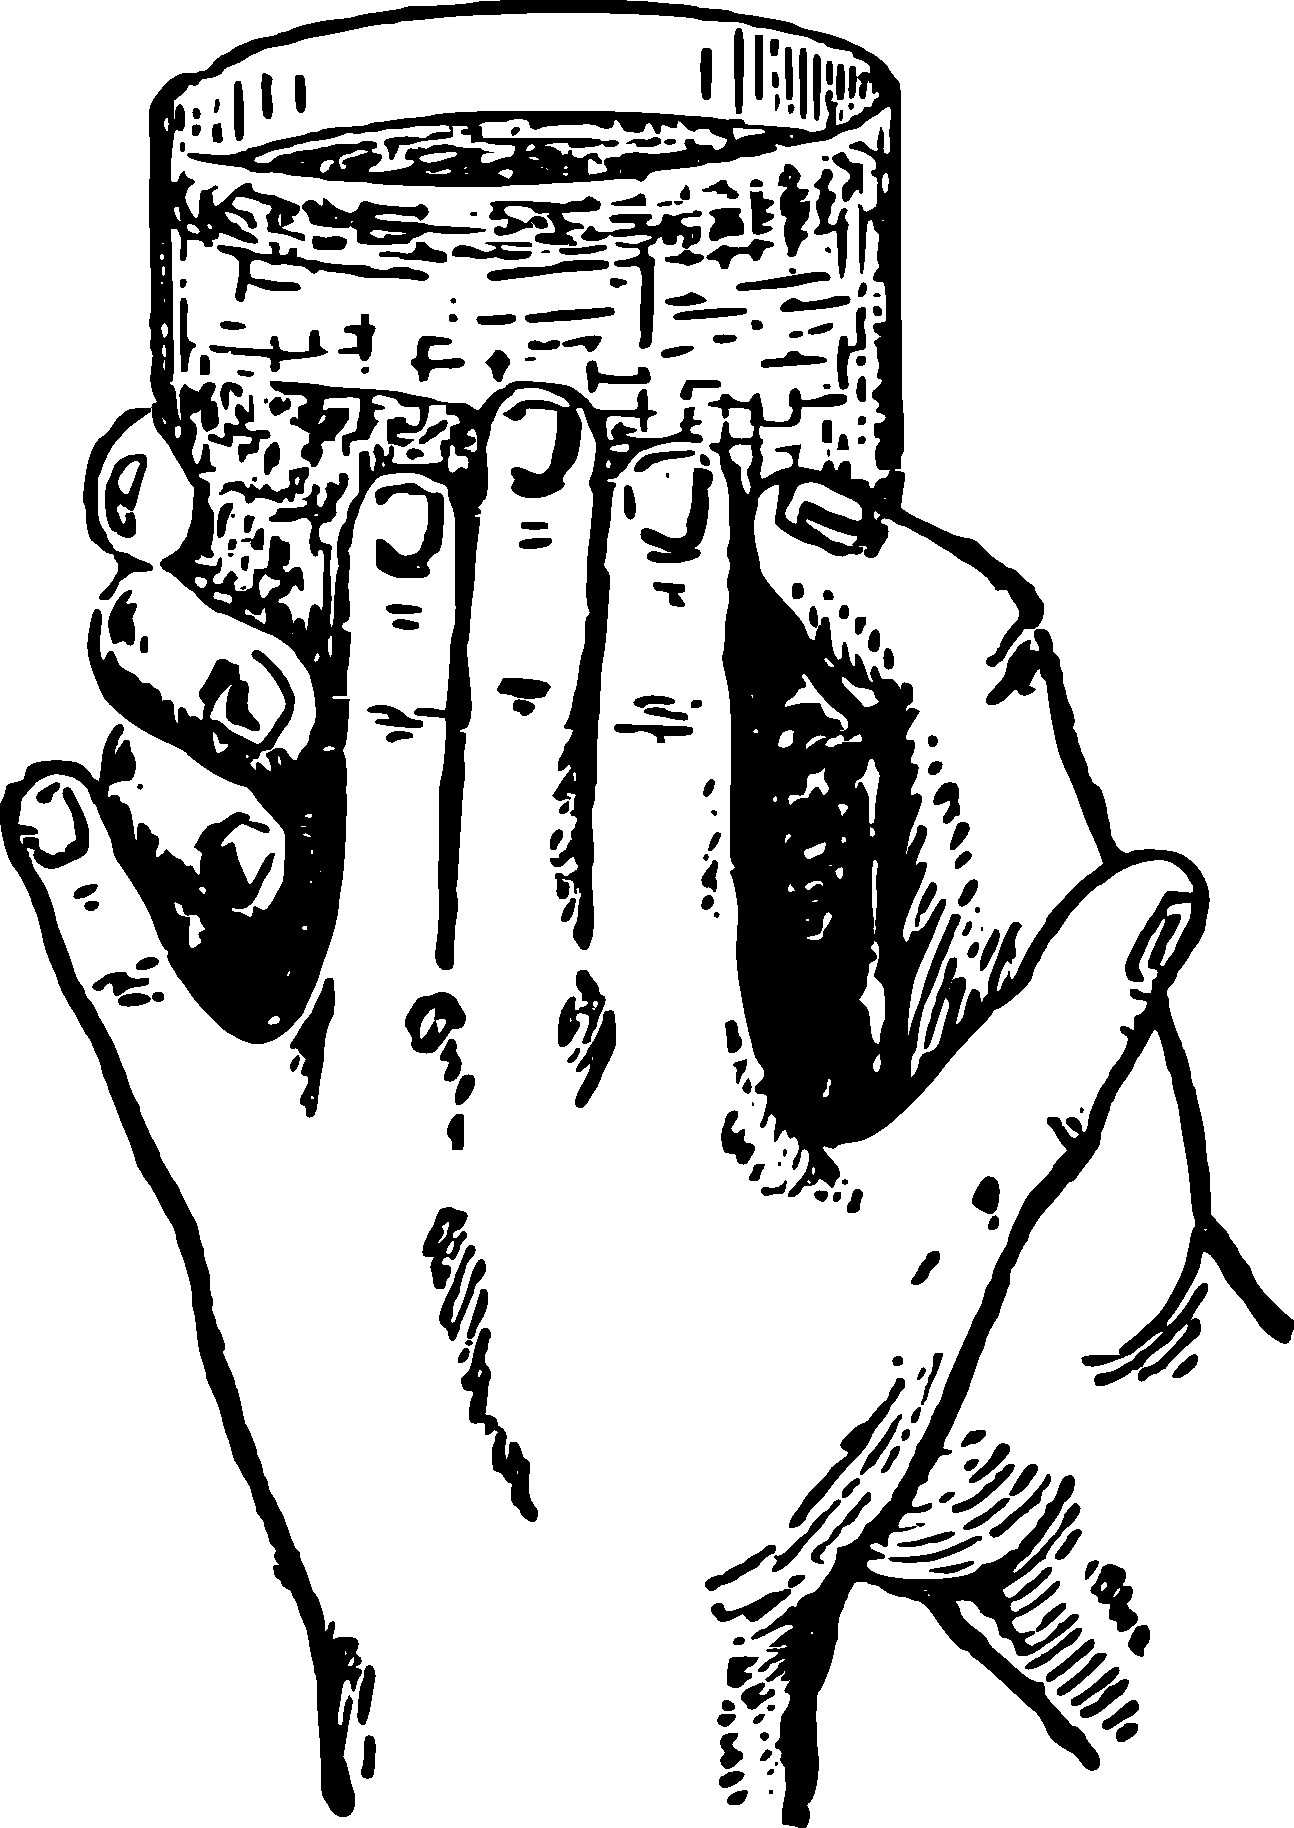
\includegraphics[width=0.35\textwidth]{figures/ch-08/fig-121.pdf}
\sidecaption{Measuring the circumference of the glass with ``bare hands''.\label{fig-121}}
\end{figure}


\section{Straight Angle in the Dark}
label{sec-8.9}

\ques Returning once again to the Mayne-Reid mathematician, let's set ourselves a task: how should he have proceeded to reliably obtain a right angle? ``I placed a long rod against it (the projecting plank) so that it formed a right angle with it,'' we read in the novel. Doing this in the dark, relying only on muscular sensations, we can make quite a few mistakes. However, the boy had a way to construct a right angle much more reliably. How?

\begin{figure}[h!]
\centering
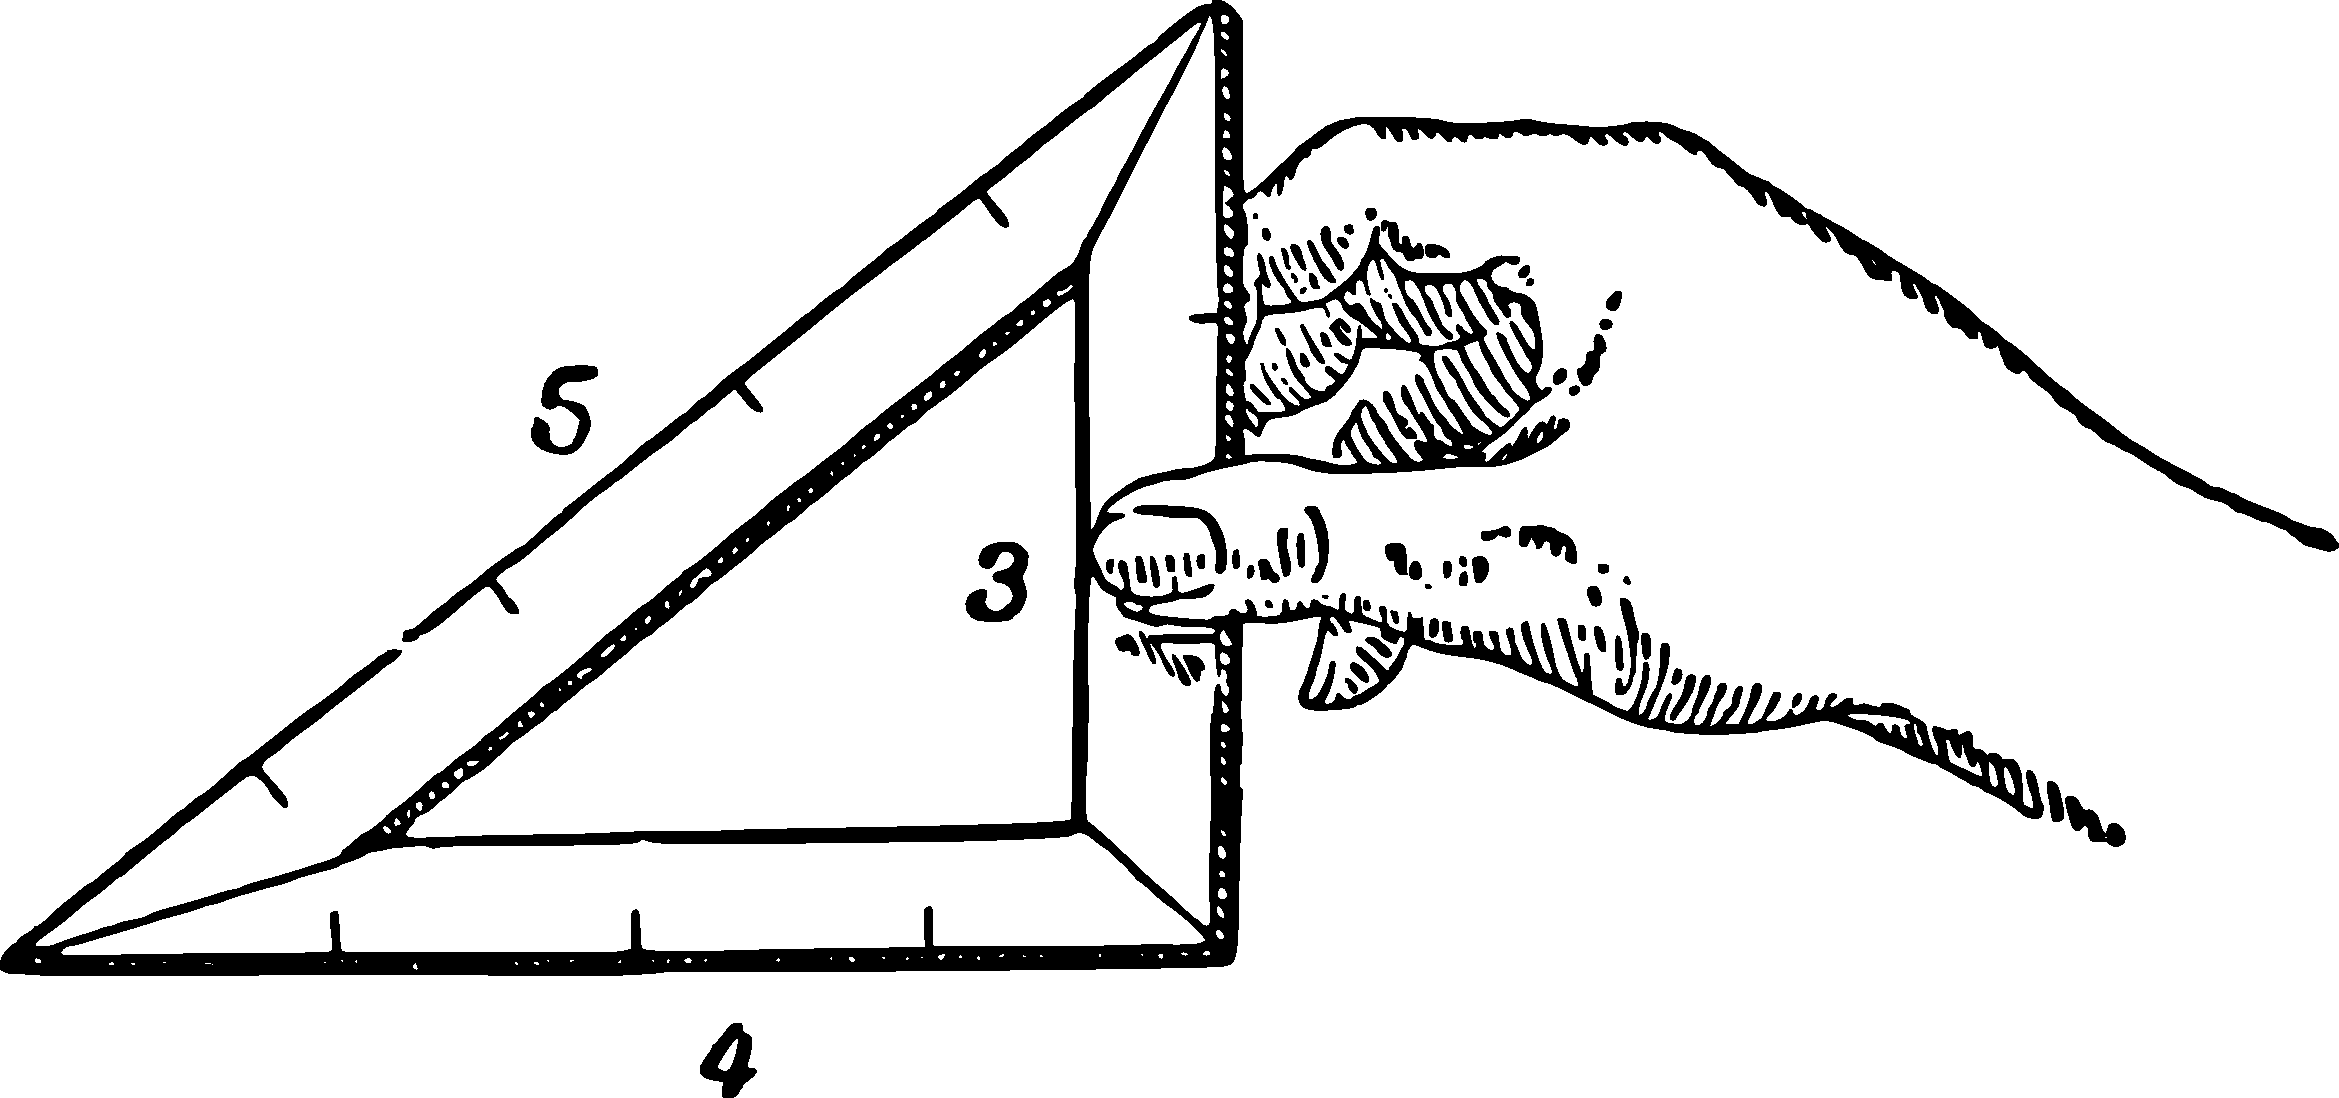
\includegraphics[width=0.8\textwidth]{figures/ch-08/fig-122.pdf}
\sidecaption[][-2cm]{The simplest right-angled triangle, the lengths of whose sides correspond to these numbers.\label{fig-122}}
\end{figure}

\ans One should resort to using the Pythagorean theorem and construct a triangle from the planks, giving its sides such lengths that the triangle becomes rectangular. The simplest way to do this is to take planks with lengths of 3, 4, and 5 arbitrary equal segments (see \figr{fig-122}).





This is an ancient Egyptian method used in the land of pyramids thousands of years ago. However, even in our days, this method is often used in construction work.

\vspace{2cm}

\begin{center}
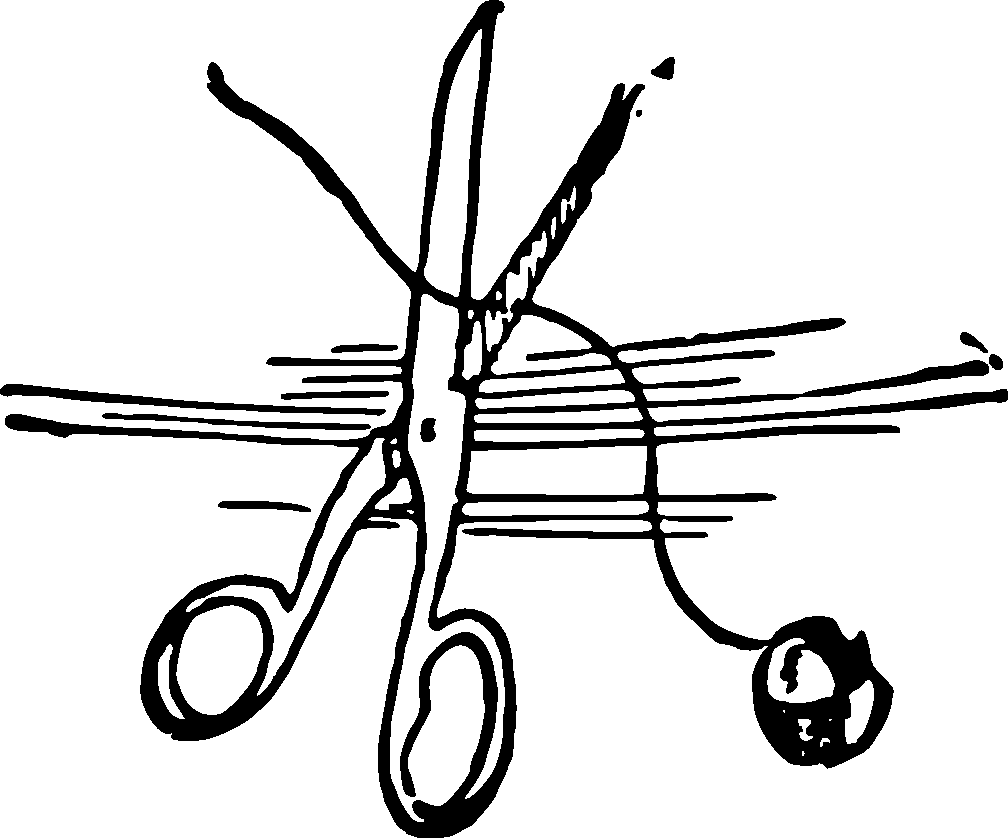
\includegraphics[width=0.3\textwidth]{figures/ch-08/fig-ch-08-tail.pdf}
\end{center}


















